\chapter{Results}

This chapter describes our use of \ac{CNN} to denoise images from the \ac{NIND}. The first section describes our suggested methods to handle the \ac{NIND} dataset. The \ac{CNN} Denoiser section first describes the various conventional network configurations we have worked with along with the Experimental results. The \ac{GAN} Denoiser section then describes our work and the results associated with (c)\ac{GAN} networks which require more experimental work and fine-tuning. 

\section{Dataset usage}\label{sec:Dataset Usage}
The \ac{NIND} is cropped in advance to speed up loading times. A crop size of 128x128 pixels was found to work well for training and larger crops did not significantly affect performance. We found that the border is most often corrupted in a U-Net model. Some network architectures perform better when required to learn to model entire crops down to their border, but it typically takes a lot of resources to get to that point and the result often still shows a grid pattern when the crops are stitched back together. We use a ``useful crop size" that is 0.75 the size of the actual crop size for U-Net models and approximately 0.875 with other architectures so that only the central part of a crop is used for stitching as well as for computing the loss. A script that crops the dataset in such overlapping blocks is provided for this purpose.

An epoch consists of training the model on every crop of any ISO value for every scene, that is, a random ISO value is fed every time a crop is loaded, therefore it takes several epochs for the model to train on all of the available data. The ground-truth is also selected randomly when multiple ones are available and basic data augmentation (rotation and/or translation) is performed.

\section{CNN Denoiser}\label{sec:CNN Denoiser}
%\subsubsection{Models}
We initially trained a DnCNN \cite{dncnn} model on our data. This model attained satisfying performance when trained to model the latent clean image instead of modeling the noise. It was further improved by using a convolution filter size of 5x5 instead of 3x3. The second architecture tested was a \ac{RED-Net} \cite{rednet} with 22-layers and a filter size of 5x5. This model obtained very good performance, albeit with an impractical runtime and memory use. We settled on a U-Net \cite{unet} architecture which provides slightly better performance with significantly lower runtime and memory use.

%\subsection{Experimental results}

We compared the performance obtained with the following methods:

\begin{enumerate}
\itemsep0em 
  \item\label{exp:nindxt1} U-Net trained on \ac{NIND} (X-T1 subset):\newline
  This model encompasses the main part of our dataset.
  \item\label{exp:sidd} U-Net trained on \ac{SIDD} (320 provided image pairs):\newline
  Compare the performance obtained using our dataset with 320 images from the \ac{SIDD} (Smartphone Image Denoising Dataset) \cite{sidd} which were made available for the 2019 NTIRE denoising challenge.
  \item\label{exp:bm3d} \ac{BM3D} \cite{bm3d} ( \cite{bm3d-gpu} implementation) with $\sigma$ = \{5, 10, 20, 30, 40, 50, 60, 70, 80, 90, 93, 95, 97, 99\}\footnote{\label{sigmanote}We test every $\sigma$ value mentioned in Methods \ref{exp:bm3d} and \ref{exp:nindart} and report the value which yields the highest \ac{SSIM} for each test image.}:\newline
  BM3D has been ubiquitously used as a reference in non-learning based image denoising.
\end{enumerate}
In addition to the aforementioned reference methods, we consider the following experiments:
\begin{enumerate}
\itemsep0em 
\setcounter{enumi}{3}
  \item\label{exp:nindall}   U-Net trained on \ac{NIND} (dataset composed of the union of \ac{X-T1} and \ac{C500D} training scenes; 89.5 \% and 10.5 \%, respectively):\newline
  When tested on a \ac{C500D} image, this method can be compared with the first reference method to determine whether training on images acquired with the test image sensor helps or not, thereby assessing the generalization capabilities of our reference model to different sensors.  In addition, it shows whether adding data from a different sensor negatively affects performance.
  \item\label{exp:nindsidd} U-Net trained on the union of \ac{NIND}:\ac{X-T1}, \ac{NIND}:\ac{C500D} scenes) and \ac{SIDD} (320 pairs); 20.5 \%, 2.4 \%, and 77.1 \% respectively:\newline
  This model shows the performance impact of adding a wildly different type of noise to the training data.
  \item\label{exp:nind6400} U-Net trained on \ac{NIND} (\ac{X-T1} subset, ISO6400 noise only instead of random ISO sample):\newline
  This experiment tests whether a model trained for blind denoising performs significantly worse than one trained for a specific ISO value.
  \item\label{exp:nindart} U-Net trained on \ac{NIND} (\ac{X-T1} subset) with artificial gaussian noise added to the ground-truth. $\sigma$ = \{[1,55], [1,60], [1,80], [1,95]\}\footnoteref{sigmanote}:\newline
  This experiment compares the performance obtained by a model trained on our real data to the widely applied approach of applying synthetic gaussian noise to clean images.
  \item\label{exp:nindmakenoise} U-Net trained to reconstruct the noise on \ac{NIND} (\ac{X-T1} subset):\newline
  We applied the residual learning strategy proposed in \cite{dncnn} by training a model that reconstructs the noise and subtracts it from the image.
  \item\label{exp:nindred} \ac{RED-Net} \cite{rednet} trained on \ac{NIND} (\ac{X-T1} subset):\newline
  This uses the same data as Method \ref{exp:nindxt1} with a different network architecture

\end{enumerate}

\begin{table*}[!htbp]
\centering
\resizebox{1\linewidth}{!}{
\begin{tabular}{l|llllllllll}
\ul{ISO value}                      & \ul{ISO200}   & \ul{ISO250}   & \ul{ISO500}   & \ul{ISO2500}  & \ul{ISO4000}  & \ul{ISO6400}  & \ul{High ISO} \\ \hline
Number of images                     & 5              & 3              & 2              & 2              & 2              & 5              & 9              \\ \hline
Noisy                                & \textbf{1.000} & 0.907          & 0.853          & 0.784          & 0.687          & 0.578          & 0.311          \\ \hline
NIND:X-T1 (U-Net)                     & 0.949          & \textbf{0.929} & \textbf{0.920} & \textbf{0.912} & \textbf{0.900} & \textbf{0.893} & \textbf{0.851} \\ \hline
SIDD (U-Net)                          & 0.906          & 0.907          & 0.904          & 0.864          & 0.882          & 0.860          & 0.814          \\ \hline
BM3D                                 & 0.941          & \textbf{0.925} & 0.913          & 0.875          & 0.870          & 0.852          & 0.785          \\ \hline
\ac{NIND}:X-T1+C500D (U-Net)               & 0.949          & \textbf{0.929} & \textbf{0.920} & \textbf{0.912} & \textbf{0.899} & \textbf{0.893} & \textbf{0.851} \\ \hline
\ac{NIND}:X-T1+C500D + \ac{SIDD} (U-Net)        & 0.947          & \textbf{0.928} & \textbf{0.919} & \textbf{0.910} & \textbf{0.898} & \textbf{0.892} & \textbf{0.850} \\ \hline
NIND:X-T1 ISO6400 only (U-Net)        & 0.919          & 0.915          & 0.911          & \textbf{0.907} & \textbf{0.901} & \textbf{0.894} & 0.821          \\ \hline
Reconstruct noise on NIND:X-T1 (U-Net)      & 0.950          & \textbf{0.926} & 0.914          & 0.901          & 0.876          & 0.840          & 0.664          \\ \hline
Artificial noise on NIND:X-T1 (U-Net) & 0.963          & 0.920          & 0.899          & 0.880          & 0.810          & 0.769          & 0.531          \\ \hline
NIND:X-T1 (\ac{RED-Net})                   & 0.940          & 0.923          & 0.915          & \textbf{0.907} & 0.892          & \textbf{0.886} & 0.842          \\ \hline
\end{tabular}%
}\caption[Average \acs{SSIM} index on 5 \acs{NIND}:\acs{X-T1} denoised scenes]{Average \acs{SSIM} index on 5 \acs{NIND}:\acs{X-T1} denoised scenes (ursulines-building, stefantiek, CourtineDeVillersDebris, MuseeL-Bobo, ursulines-red). The best performing models (to within two significant digits) are marked in bold.}
\label{tableNINDXT1}
\end{table*}

\begin{table*}[!htbp]
\centering
\resizebox{1\linewidth}{!}{%
\begin{tabular}{l|lllllll}
\ul{ISO value}                            & \ul{ISO100}   & \ul{ISO200}   & \ul{ISO400}   & \ul{ISO800}   & \ul{ISO1600}  & \ul{ISO3200}  & \ul{High ISO} \\ \hline
{Noisy}                                & \textbf{1.000} & 0.814          & 0.754          & 0.660          & 0.550          & 0.401          & 0.172          \\ \hline
{NIND:X-T1 (U-Net)}                     & 0.911          & \textbf{0.901} & \textbf{0.898} & \textbf{0.896} & \textbf{0.893} & \textbf{0.887} & \textbf{0.868} \\ \hline
{SIDD (U-Net)}                          & 0.894         & 0.892           & 0.890          & 0.889          & 0.885  & 0.876          & 0.850          \\ \hline
{BM3D}                                 & 0.921          & 0.890          & 0.884          & 0.877          & 0.871          & 0.860          & 0.813          \\ \hline
{\ac{NIND}:\ac{X-T1}+\ac{C500D} (U-Net)}               & 0.911          & \textbf{0.901} & \textbf{0.899} & \textbf{0.896} & \textbf{0.894} & \textbf{0.888} & \textbf{0.872} \\ \hline
{\ac{NIND}:\ac{X-T1}+\ac{C500D} + \ac{SIDD} (U-Net)}        & 0.912          & \textbf{0.901} & \textbf{0.899} & \textbf{0.896} & \textbf{0.893} & \textbf{0.888} & \textbf{0.871} \\ \hline
{\ac{NIND}:\ac{X-T1} ISO6400 only (U-Net)}        & 0.899          & \textbf{0.897} & \textbf{0.896} & 0.894          & \textbf{0.892} & \textbf{0.886} & \textbf{0.865} \\ \hline
{Reconstruct noise on \ac{NIND}:\ac{X-T1} (U-Net)}      & 0.908          & 0.895          & 0.887          & 0.875          & 0.855          & 0.807          & 0.617          \\ \hline
{Artificial noise on \ac{NIND}:\ac{X-T1} (U-Net)} & 0.946          & 0.879          & 0.864          & 0.836          & 0.802          & 0.716          & 0.430          \\ \hline
\end{tabular}%
}\caption{\acs{SSIM} index on \acs{NIND}:\acs{C500D} denoised set MuseeL-Bobo-C500D}
\label{tableNINDXT1onBoboC500D}
\end{table*}

\begin{table*}[!htbp]
\centering
\resizebox{1\linewidth}{!}{%
\begin{tabular}{l|lllllll}
\ul{ISO value}                       & \ul{ISO100}   & \ul{ISO200}   & \ul{ISO400}   & \ul{ISO800}   & \ul{ISO1600}  & \ul{ISO3200}  & \ul{High ISO} \\ \hline
\ul{\# images}                       & 13             & 9              & 9              & 9              & 8              & 10             & 9              \\ \hline
\ul{Noisy}                           & \textbf{0.954} & 0.766          & 0.707          & 0.619          & 0.501          & 0.380          & 0.220          \\ \hline
\ul{NIND:X-T1 (U-Net)}                & 0.878          & \textbf{0.856} & \textbf{0.854} & \textbf{0.848} & \textbf{0.845} & \textbf{0.834} & \textbf{0.805} \\ \hline
\ul{SIDD (U-Net)}                     & 0.851         & 0.838          & 0.837          & 0.834          & 0.830          & 0.813          & 0.774          \\ \hline
\ul{BM3D}                            & 0.899          & 0.836          & 0.825          & 0.816          & 0.811          & 0.789          & 0.749          \\ \hline
\ul{NIND:X-T1 ISO6400 only (U-Net)}   & 0.857          & 0.847          & \textbf{0.847} & 0.845          & \textbf{0.843} & \textbf{0.834} & 0.802          \\ \hline
\ul{Reconstruct noise on NIND:X-T1 (U-Net)} & 0.878          & 0.845          & 0.835          & 0.814          & 0.785          & 0.725          & 0.604          \\ \hline
\end{tabular}%
}\caption{Average \acs{SSIM} index on 10 \acs{NIND}:\acs{C500D} scenes denoised with models trained on \acs{NIND}:\acs{X-T1} or with \acs{BM3D}}
\label{tableXT1onC500D}
\end{table*}

\begin{figure}[!htbp]
\centering
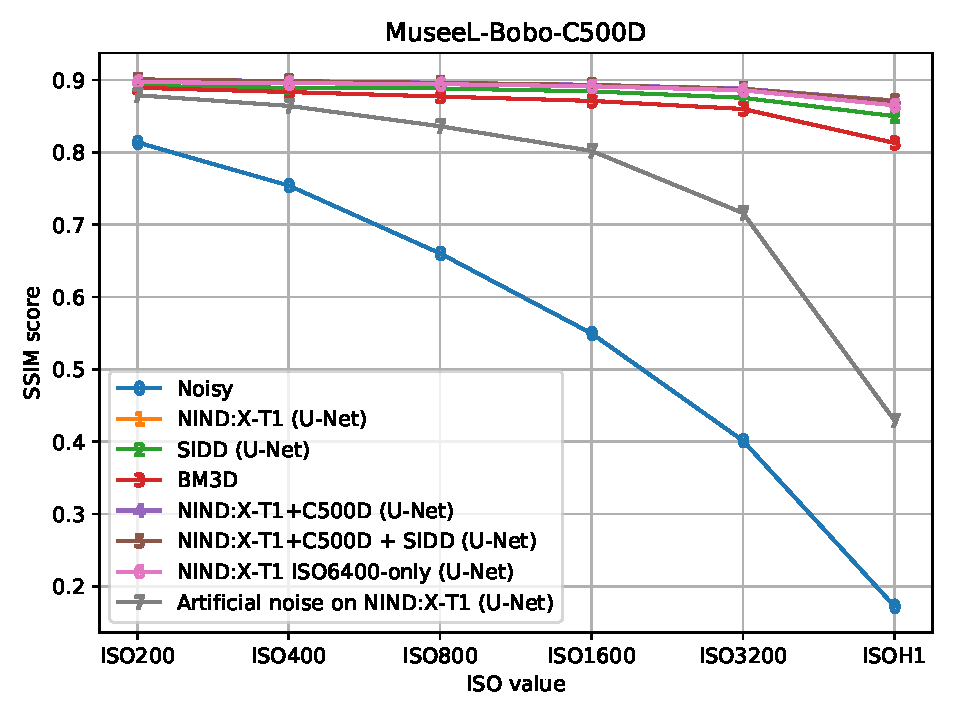
\includegraphics[width=1\linewidth]{gfx/graphs/boboc500d.pdf}
%%% Creator: Matplotlib, PGF backend
%%
%% To include the figure in your LaTeX document, write
%%   \input{<filename>.pgf}
%%
%% Make sure the required packages are loaded in your preamble
%%   \usepackage{pgf}
%%
%% Figures using additional raster images can only be included by \input if
%% they are in the same directory as the main LaTeX file. For loading figures
%% from other directories you can use the `import` package
%%   \usepackage{import}
%% and then include the figures with
%%   \import{<path to file>}{<filename>.pgf}
%%
%% Matplotlib used the following preamble
%%   \usepackage{fontspec}
%%   \setmainfont{DejaVuSerif.ttf}[Path=/usr/lib/python3.7/site-packages/matplotlib/mpl-data/fonts/ttf/]
%%   \setsansfont{DejaVuSans.ttf}[Path=/usr/lib/python3.7/site-packages/matplotlib/mpl-data/fonts/ttf/]
%%   \setmonofont{DejaVuSansMono.ttf}[Path=/usr/lib/python3.7/site-packages/matplotlib/mpl-data/fonts/ttf/]
%%
\begingroup%
\makeatletter%
\begin{pgfpicture}%
\pgfpathrectangle{\pgfpointorigin}{\pgfqpoint{38.400000in}{20.430000in}}%
\pgfusepath{use as bounding box, clip}%
\begin{pgfscope}%
\pgfsetbuttcap%
\pgfsetmiterjoin%
\definecolor{currentfill}{rgb}{1.000000,1.000000,1.000000}%
\pgfsetfillcolor{currentfill}%
\pgfsetlinewidth{0.000000pt}%
\definecolor{currentstroke}{rgb}{1.000000,1.000000,1.000000}%
\pgfsetstrokecolor{currentstroke}%
\pgfsetdash{}{0pt}%
\pgfpathmoveto{\pgfqpoint{0.000000in}{0.000000in}}%
\pgfpathlineto{\pgfqpoint{38.400000in}{0.000000in}}%
\pgfpathlineto{\pgfqpoint{38.400000in}{20.430000in}}%
\pgfpathlineto{\pgfqpoint{0.000000in}{20.430000in}}%
\pgfpathclose%
\pgfusepath{fill}%
\end{pgfscope}%
\begin{pgfscope}%
\pgfsetbuttcap%
\pgfsetmiterjoin%
\definecolor{currentfill}{rgb}{1.000000,1.000000,1.000000}%
\pgfsetfillcolor{currentfill}%
\pgfsetlinewidth{0.000000pt}%
\definecolor{currentstroke}{rgb}{0.000000,0.000000,0.000000}%
\pgfsetstrokecolor{currentstroke}%
\pgfsetstrokeopacity{0.000000}%
\pgfsetdash{}{0pt}%
\pgfpathmoveto{\pgfqpoint{0.662778in}{0.582778in}}%
\pgfpathlineto{\pgfqpoint{38.215000in}{0.582778in}}%
\pgfpathlineto{\pgfqpoint{38.215000in}{20.076667in}}%
\pgfpathlineto{\pgfqpoint{0.662778in}{20.076667in}}%
\pgfpathclose%
\pgfusepath{fill}%
\end{pgfscope}%
\begin{pgfscope}%
\pgfpathrectangle{\pgfqpoint{0.662778in}{0.582778in}}{\pgfqpoint{37.552222in}{19.493889in}}%
\pgfusepath{clip}%
\pgfsetrectcap%
\pgfsetroundjoin%
\pgfsetlinewidth{0.803000pt}%
\definecolor{currentstroke}{rgb}{0.690196,0.690196,0.690196}%
\pgfsetstrokecolor{currentstroke}%
\pgfsetdash{}{0pt}%
\pgfpathmoveto{\pgfqpoint{2.369697in}{0.582778in}}%
\pgfpathlineto{\pgfqpoint{2.369697in}{20.076667in}}%
\pgfusepath{stroke}%
\end{pgfscope}%
\begin{pgfscope}%
\pgfsetbuttcap%
\pgfsetroundjoin%
\definecolor{currentfill}{rgb}{0.000000,0.000000,0.000000}%
\pgfsetfillcolor{currentfill}%
\pgfsetlinewidth{0.803000pt}%
\definecolor{currentstroke}{rgb}{0.000000,0.000000,0.000000}%
\pgfsetstrokecolor{currentstroke}%
\pgfsetdash{}{0pt}%
\pgfsys@defobject{currentmarker}{\pgfqpoint{0.000000in}{-0.048611in}}{\pgfqpoint{0.000000in}{0.000000in}}{%
\pgfpathmoveto{\pgfqpoint{0.000000in}{0.000000in}}%
\pgfpathlineto{\pgfqpoint{0.000000in}{-0.048611in}}%
\pgfusepath{stroke,fill}%
}%
\begin{pgfscope}%
\pgfsys@transformshift{2.369697in}{0.582778in}%
\pgfsys@useobject{currentmarker}{}%
\end{pgfscope}%
\end{pgfscope}%
\begin{pgfscope}%
\definecolor{textcolor}{rgb}{0.000000,0.000000,0.000000}%
\pgfsetstrokecolor{textcolor}%
\pgfsetfillcolor{textcolor}%
\pgftext[x=2.369697in,y=0.485556in,,top]{\color{textcolor}\sffamily\fontsize{10.000000}{12.000000}\selectfont ISO200}%
\end{pgfscope}%
\begin{pgfscope}%
\pgfpathrectangle{\pgfqpoint{0.662778in}{0.582778in}}{\pgfqpoint{37.552222in}{19.493889in}}%
\pgfusepath{clip}%
\pgfsetrectcap%
\pgfsetroundjoin%
\pgfsetlinewidth{0.803000pt}%
\definecolor{currentstroke}{rgb}{0.690196,0.690196,0.690196}%
\pgfsetstrokecolor{currentstroke}%
\pgfsetdash{}{0pt}%
\pgfpathmoveto{\pgfqpoint{9.197374in}{0.582778in}}%
\pgfpathlineto{\pgfqpoint{9.197374in}{20.076667in}}%
\pgfusepath{stroke}%
\end{pgfscope}%
\begin{pgfscope}%
\pgfsetbuttcap%
\pgfsetroundjoin%
\definecolor{currentfill}{rgb}{0.000000,0.000000,0.000000}%
\pgfsetfillcolor{currentfill}%
\pgfsetlinewidth{0.803000pt}%
\definecolor{currentstroke}{rgb}{0.000000,0.000000,0.000000}%
\pgfsetstrokecolor{currentstroke}%
\pgfsetdash{}{0pt}%
\pgfsys@defobject{currentmarker}{\pgfqpoint{0.000000in}{-0.048611in}}{\pgfqpoint{0.000000in}{0.000000in}}{%
\pgfpathmoveto{\pgfqpoint{0.000000in}{0.000000in}}%
\pgfpathlineto{\pgfqpoint{0.000000in}{-0.048611in}}%
\pgfusepath{stroke,fill}%
}%
\begin{pgfscope}%
\pgfsys@transformshift{9.197374in}{0.582778in}%
\pgfsys@useobject{currentmarker}{}%
\end{pgfscope}%
\end{pgfscope}%
\begin{pgfscope}%
\definecolor{textcolor}{rgb}{0.000000,0.000000,0.000000}%
\pgfsetstrokecolor{textcolor}%
\pgfsetfillcolor{textcolor}%
\pgftext[x=9.197374in,y=0.485556in,,top]{\color{textcolor}\sffamily\fontsize{10.000000}{12.000000}\selectfont ISO400}%
\end{pgfscope}%
\begin{pgfscope}%
\pgfpathrectangle{\pgfqpoint{0.662778in}{0.582778in}}{\pgfqpoint{37.552222in}{19.493889in}}%
\pgfusepath{clip}%
\pgfsetrectcap%
\pgfsetroundjoin%
\pgfsetlinewidth{0.803000pt}%
\definecolor{currentstroke}{rgb}{0.690196,0.690196,0.690196}%
\pgfsetstrokecolor{currentstroke}%
\pgfsetdash{}{0pt}%
\pgfpathmoveto{\pgfqpoint{16.025051in}{0.582778in}}%
\pgfpathlineto{\pgfqpoint{16.025051in}{20.076667in}}%
\pgfusepath{stroke}%
\end{pgfscope}%
\begin{pgfscope}%
\pgfsetbuttcap%
\pgfsetroundjoin%
\definecolor{currentfill}{rgb}{0.000000,0.000000,0.000000}%
\pgfsetfillcolor{currentfill}%
\pgfsetlinewidth{0.803000pt}%
\definecolor{currentstroke}{rgb}{0.000000,0.000000,0.000000}%
\pgfsetstrokecolor{currentstroke}%
\pgfsetdash{}{0pt}%
\pgfsys@defobject{currentmarker}{\pgfqpoint{0.000000in}{-0.048611in}}{\pgfqpoint{0.000000in}{0.000000in}}{%
\pgfpathmoveto{\pgfqpoint{0.000000in}{0.000000in}}%
\pgfpathlineto{\pgfqpoint{0.000000in}{-0.048611in}}%
\pgfusepath{stroke,fill}%
}%
\begin{pgfscope}%
\pgfsys@transformshift{16.025051in}{0.582778in}%
\pgfsys@useobject{currentmarker}{}%
\end{pgfscope}%
\end{pgfscope}%
\begin{pgfscope}%
\definecolor{textcolor}{rgb}{0.000000,0.000000,0.000000}%
\pgfsetstrokecolor{textcolor}%
\pgfsetfillcolor{textcolor}%
\pgftext[x=16.025051in,y=0.485556in,,top]{\color{textcolor}\sffamily\fontsize{10.000000}{12.000000}\selectfont ISO800}%
\end{pgfscope}%
\begin{pgfscope}%
\pgfpathrectangle{\pgfqpoint{0.662778in}{0.582778in}}{\pgfqpoint{37.552222in}{19.493889in}}%
\pgfusepath{clip}%
\pgfsetrectcap%
\pgfsetroundjoin%
\pgfsetlinewidth{0.803000pt}%
\definecolor{currentstroke}{rgb}{0.690196,0.690196,0.690196}%
\pgfsetstrokecolor{currentstroke}%
\pgfsetdash{}{0pt}%
\pgfpathmoveto{\pgfqpoint{22.852727in}{0.582778in}}%
\pgfpathlineto{\pgfqpoint{22.852727in}{20.076667in}}%
\pgfusepath{stroke}%
\end{pgfscope}%
\begin{pgfscope}%
\pgfsetbuttcap%
\pgfsetroundjoin%
\definecolor{currentfill}{rgb}{0.000000,0.000000,0.000000}%
\pgfsetfillcolor{currentfill}%
\pgfsetlinewidth{0.803000pt}%
\definecolor{currentstroke}{rgb}{0.000000,0.000000,0.000000}%
\pgfsetstrokecolor{currentstroke}%
\pgfsetdash{}{0pt}%
\pgfsys@defobject{currentmarker}{\pgfqpoint{0.000000in}{-0.048611in}}{\pgfqpoint{0.000000in}{0.000000in}}{%
\pgfpathmoveto{\pgfqpoint{0.000000in}{0.000000in}}%
\pgfpathlineto{\pgfqpoint{0.000000in}{-0.048611in}}%
\pgfusepath{stroke,fill}%
}%
\begin{pgfscope}%
\pgfsys@transformshift{22.852727in}{0.582778in}%
\pgfsys@useobject{currentmarker}{}%
\end{pgfscope}%
\end{pgfscope}%
\begin{pgfscope}%
\definecolor{textcolor}{rgb}{0.000000,0.000000,0.000000}%
\pgfsetstrokecolor{textcolor}%
\pgfsetfillcolor{textcolor}%
\pgftext[x=22.852727in,y=0.485556in,,top]{\color{textcolor}\sffamily\fontsize{10.000000}{12.000000}\selectfont ISO1600}%
\end{pgfscope}%
\begin{pgfscope}%
\pgfpathrectangle{\pgfqpoint{0.662778in}{0.582778in}}{\pgfqpoint{37.552222in}{19.493889in}}%
\pgfusepath{clip}%
\pgfsetrectcap%
\pgfsetroundjoin%
\pgfsetlinewidth{0.803000pt}%
\definecolor{currentstroke}{rgb}{0.690196,0.690196,0.690196}%
\pgfsetstrokecolor{currentstroke}%
\pgfsetdash{}{0pt}%
\pgfpathmoveto{\pgfqpoint{29.680404in}{0.582778in}}%
\pgfpathlineto{\pgfqpoint{29.680404in}{20.076667in}}%
\pgfusepath{stroke}%
\end{pgfscope}%
\begin{pgfscope}%
\pgfsetbuttcap%
\pgfsetroundjoin%
\definecolor{currentfill}{rgb}{0.000000,0.000000,0.000000}%
\pgfsetfillcolor{currentfill}%
\pgfsetlinewidth{0.803000pt}%
\definecolor{currentstroke}{rgb}{0.000000,0.000000,0.000000}%
\pgfsetstrokecolor{currentstroke}%
\pgfsetdash{}{0pt}%
\pgfsys@defobject{currentmarker}{\pgfqpoint{0.000000in}{-0.048611in}}{\pgfqpoint{0.000000in}{0.000000in}}{%
\pgfpathmoveto{\pgfqpoint{0.000000in}{0.000000in}}%
\pgfpathlineto{\pgfqpoint{0.000000in}{-0.048611in}}%
\pgfusepath{stroke,fill}%
}%
\begin{pgfscope}%
\pgfsys@transformshift{29.680404in}{0.582778in}%
\pgfsys@useobject{currentmarker}{}%
\end{pgfscope}%
\end{pgfscope}%
\begin{pgfscope}%
\definecolor{textcolor}{rgb}{0.000000,0.000000,0.000000}%
\pgfsetstrokecolor{textcolor}%
\pgfsetfillcolor{textcolor}%
\pgftext[x=29.680404in,y=0.485556in,,top]{\color{textcolor}\sffamily\fontsize{10.000000}{12.000000}\selectfont ISO3200}%
\end{pgfscope}%
\begin{pgfscope}%
\pgfpathrectangle{\pgfqpoint{0.662778in}{0.582778in}}{\pgfqpoint{37.552222in}{19.493889in}}%
\pgfusepath{clip}%
\pgfsetrectcap%
\pgfsetroundjoin%
\pgfsetlinewidth{0.803000pt}%
\definecolor{currentstroke}{rgb}{0.690196,0.690196,0.690196}%
\pgfsetstrokecolor{currentstroke}%
\pgfsetdash{}{0pt}%
\pgfpathmoveto{\pgfqpoint{36.508081in}{0.582778in}}%
\pgfpathlineto{\pgfqpoint{36.508081in}{20.076667in}}%
\pgfusepath{stroke}%
\end{pgfscope}%
\begin{pgfscope}%
\pgfsetbuttcap%
\pgfsetroundjoin%
\definecolor{currentfill}{rgb}{0.000000,0.000000,0.000000}%
\pgfsetfillcolor{currentfill}%
\pgfsetlinewidth{0.803000pt}%
\definecolor{currentstroke}{rgb}{0.000000,0.000000,0.000000}%
\pgfsetstrokecolor{currentstroke}%
\pgfsetdash{}{0pt}%
\pgfsys@defobject{currentmarker}{\pgfqpoint{0.000000in}{-0.048611in}}{\pgfqpoint{0.000000in}{0.000000in}}{%
\pgfpathmoveto{\pgfqpoint{0.000000in}{0.000000in}}%
\pgfpathlineto{\pgfqpoint{0.000000in}{-0.048611in}}%
\pgfusepath{stroke,fill}%
}%
\begin{pgfscope}%
\pgfsys@transformshift{36.508081in}{0.582778in}%
\pgfsys@useobject{currentmarker}{}%
\end{pgfscope}%
\end{pgfscope}%
\begin{pgfscope}%
\definecolor{textcolor}{rgb}{0.000000,0.000000,0.000000}%
\pgfsetstrokecolor{textcolor}%
\pgfsetfillcolor{textcolor}%
\pgftext[x=36.508081in,y=0.485556in,,top]{\color{textcolor}\sffamily\fontsize{10.000000}{12.000000}\selectfont ISOH1}%
\end{pgfscope}%
\begin{pgfscope}%
\definecolor{textcolor}{rgb}{0.000000,0.000000,0.000000}%
\pgfsetstrokecolor{textcolor}%
\pgfsetfillcolor{textcolor}%
\pgftext[x=19.438889in,y=0.295587in,,top]{\color{textcolor}\sffamily\fontsize{10.000000}{12.000000}\selectfont ISO value}%
\end{pgfscope}%
\begin{pgfscope}%
\pgfpathrectangle{\pgfqpoint{0.662778in}{0.582778in}}{\pgfqpoint{37.552222in}{19.493889in}}%
\pgfusepath{clip}%
\pgfsetrectcap%
\pgfsetroundjoin%
\pgfsetlinewidth{0.803000pt}%
\definecolor{currentstroke}{rgb}{0.690196,0.690196,0.690196}%
\pgfsetstrokecolor{currentstroke}%
\pgfsetdash{}{0pt}%
\pgfpathmoveto{\pgfqpoint{0.662778in}{8.491192in}}%
\pgfpathlineto{\pgfqpoint{38.215000in}{8.491192in}}%
\pgfusepath{stroke}%
\end{pgfscope}%
\begin{pgfscope}%
\pgfsetbuttcap%
\pgfsetroundjoin%
\definecolor{currentfill}{rgb}{0.000000,0.000000,0.000000}%
\pgfsetfillcolor{currentfill}%
\pgfsetlinewidth{0.803000pt}%
\definecolor{currentstroke}{rgb}{0.000000,0.000000,0.000000}%
\pgfsetstrokecolor{currentstroke}%
\pgfsetdash{}{0pt}%
\pgfsys@defobject{currentmarker}{\pgfqpoint{-0.048611in}{0.000000in}}{\pgfqpoint{0.000000in}{0.000000in}}{%
\pgfpathmoveto{\pgfqpoint{0.000000in}{0.000000in}}%
\pgfpathlineto{\pgfqpoint{-0.048611in}{0.000000in}}%
\pgfusepath{stroke,fill}%
}%
\begin{pgfscope}%
\pgfsys@transformshift{0.662778in}{8.491192in}%
\pgfsys@useobject{currentmarker}{}%
\end{pgfscope}%
\end{pgfscope}%
\begin{pgfscope}%
\definecolor{textcolor}{rgb}{0.000000,0.000000,0.000000}%
\pgfsetstrokecolor{textcolor}%
\pgfsetfillcolor{textcolor}%
\pgftext[x=0.256311in,y=8.438430in,left,base]{\color{textcolor}\sffamily\fontsize{10.000000}{12.000000}\selectfont 0.50}%
\end{pgfscope}%
\begin{pgfscope}%
\pgfpathrectangle{\pgfqpoint{0.662778in}{0.582778in}}{\pgfqpoint{37.552222in}{19.493889in}}%
\pgfusepath{clip}%
\pgfsetrectcap%
\pgfsetroundjoin%
\pgfsetlinewidth{0.803000pt}%
\definecolor{currentstroke}{rgb}{0.690196,0.690196,0.690196}%
\pgfsetstrokecolor{currentstroke}%
\pgfsetdash{}{0pt}%
\pgfpathmoveto{\pgfqpoint{0.662778in}{17.887141in}}%
\pgfpathlineto{\pgfqpoint{38.215000in}{17.887141in}}%
\pgfusepath{stroke}%
\end{pgfscope}%
\begin{pgfscope}%
\pgfsetbuttcap%
\pgfsetroundjoin%
\definecolor{currentfill}{rgb}{0.000000,0.000000,0.000000}%
\pgfsetfillcolor{currentfill}%
\pgfsetlinewidth{0.803000pt}%
\definecolor{currentstroke}{rgb}{0.000000,0.000000,0.000000}%
\pgfsetstrokecolor{currentstroke}%
\pgfsetdash{}{0pt}%
\pgfsys@defobject{currentmarker}{\pgfqpoint{-0.048611in}{0.000000in}}{\pgfqpoint{0.000000in}{0.000000in}}{%
\pgfpathmoveto{\pgfqpoint{0.000000in}{0.000000in}}%
\pgfpathlineto{\pgfqpoint{-0.048611in}{0.000000in}}%
\pgfusepath{stroke,fill}%
}%
\begin{pgfscope}%
\pgfsys@transformshift{0.662778in}{17.887141in}%
\pgfsys@useobject{currentmarker}{}%
\end{pgfscope}%
\end{pgfscope}%
\begin{pgfscope}%
\definecolor{textcolor}{rgb}{0.000000,0.000000,0.000000}%
\pgfsetstrokecolor{textcolor}%
\pgfsetfillcolor{textcolor}%
\pgftext[x=0.256311in,y=17.834379in,left,base]{\color{textcolor}\sffamily\fontsize{10.000000}{12.000000}\selectfont 0.90}%
\end{pgfscope}%
\begin{pgfscope}%
\pgfsetbuttcap%
\pgfsetroundjoin%
\definecolor{currentfill}{rgb}{0.000000,0.000000,0.000000}%
\pgfsetfillcolor{currentfill}%
\pgfsetlinewidth{0.602250pt}%
\definecolor{currentstroke}{rgb}{0.000000,0.000000,0.000000}%
\pgfsetstrokecolor{currentstroke}%
\pgfsetdash{}{0pt}%
\pgfsys@defobject{currentmarker}{\pgfqpoint{-0.027778in}{0.000000in}}{\pgfqpoint{0.000000in}{0.000000in}}{%
\pgfpathmoveto{\pgfqpoint{0.000000in}{0.000000in}}%
\pgfpathlineto{\pgfqpoint{-0.027778in}{0.000000in}}%
\pgfusepath{stroke,fill}%
}%
\begin{pgfscope}%
\pgfsys@transformshift{0.662778in}{2.563008in}%
\pgfsys@useobject{currentmarker}{}%
\end{pgfscope}%
\end{pgfscope}%
\begin{pgfscope}%
\definecolor{textcolor}{rgb}{0.000000,0.000000,0.000000}%
\pgfsetstrokecolor{textcolor}%
\pgfsetfillcolor{textcolor}%
\pgftext[x=0.278533in,y=2.510247in,left,base]{\color{textcolor}\sffamily\fontsize{10.000000}{12.000000}\selectfont 0.20}%
\end{pgfscope}%
\begin{pgfscope}%
\pgfsetbuttcap%
\pgfsetroundjoin%
\definecolor{currentfill}{rgb}{0.000000,0.000000,0.000000}%
\pgfsetfillcolor{currentfill}%
\pgfsetlinewidth{0.602250pt}%
\definecolor{currentstroke}{rgb}{0.000000,0.000000,0.000000}%
\pgfsetstrokecolor{currentstroke}%
\pgfsetdash{}{0pt}%
\pgfsys@defobject{currentmarker}{\pgfqpoint{-0.027778in}{0.000000in}}{\pgfqpoint{0.000000in}{0.000000in}}{%
\pgfpathmoveto{\pgfqpoint{0.000000in}{0.000000in}}%
\pgfpathlineto{\pgfqpoint{-0.027778in}{0.000000in}}%
\pgfusepath{stroke,fill}%
}%
\begin{pgfscope}%
\pgfsys@transformshift{0.662778in}{4.867908in}%
\pgfsys@useobject{currentmarker}{}%
\end{pgfscope}%
\end{pgfscope}%
\begin{pgfscope}%
\definecolor{textcolor}{rgb}{0.000000,0.000000,0.000000}%
\pgfsetstrokecolor{textcolor}%
\pgfsetfillcolor{textcolor}%
\pgftext[x=0.278533in,y=4.815147in,left,base]{\color{textcolor}\sffamily\fontsize{10.000000}{12.000000}\selectfont 0.30}%
\end{pgfscope}%
\begin{pgfscope}%
\pgfsetbuttcap%
\pgfsetroundjoin%
\definecolor{currentfill}{rgb}{0.000000,0.000000,0.000000}%
\pgfsetfillcolor{currentfill}%
\pgfsetlinewidth{0.602250pt}%
\definecolor{currentstroke}{rgb}{0.000000,0.000000,0.000000}%
\pgfsetstrokecolor{currentstroke}%
\pgfsetdash{}{0pt}%
\pgfsys@defobject{currentmarker}{\pgfqpoint{-0.027778in}{0.000000in}}{\pgfqpoint{0.000000in}{0.000000in}}{%
\pgfpathmoveto{\pgfqpoint{0.000000in}{0.000000in}}%
\pgfpathlineto{\pgfqpoint{-0.027778in}{0.000000in}}%
\pgfusepath{stroke,fill}%
}%
\begin{pgfscope}%
\pgfsys@transformshift{0.662778in}{6.757309in}%
\pgfsys@useobject{currentmarker}{}%
\end{pgfscope}%
\end{pgfscope}%
\begin{pgfscope}%
\definecolor{textcolor}{rgb}{0.000000,0.000000,0.000000}%
\pgfsetstrokecolor{textcolor}%
\pgfsetfillcolor{textcolor}%
\pgftext[x=0.278533in,y=6.704548in,left,base]{\color{textcolor}\sffamily\fontsize{10.000000}{12.000000}\selectfont 0.40}%
\end{pgfscope}%
\begin{pgfscope}%
\pgfsetbuttcap%
\pgfsetroundjoin%
\definecolor{currentfill}{rgb}{0.000000,0.000000,0.000000}%
\pgfsetfillcolor{currentfill}%
\pgfsetlinewidth{0.602250pt}%
\definecolor{currentstroke}{rgb}{0.000000,0.000000,0.000000}%
\pgfsetstrokecolor{currentstroke}%
\pgfsetdash{}{0pt}%
\pgfsys@defobject{currentmarker}{\pgfqpoint{-0.027778in}{0.000000in}}{\pgfqpoint{0.000000in}{0.000000in}}{%
\pgfpathmoveto{\pgfqpoint{0.000000in}{0.000000in}}%
\pgfpathlineto{\pgfqpoint{-0.027778in}{0.000000in}}%
\pgfusepath{stroke,fill}%
}%
\begin{pgfscope}%
\pgfsys@transformshift{0.662778in}{10.225075in}%
\pgfsys@useobject{currentmarker}{}%
\end{pgfscope}%
\end{pgfscope}%
\begin{pgfscope}%
\definecolor{textcolor}{rgb}{0.000000,0.000000,0.000000}%
\pgfsetstrokecolor{textcolor}%
\pgfsetfillcolor{textcolor}%
\pgftext[x=0.278533in,y=10.172313in,left,base]{\color{textcolor}\sffamily\fontsize{10.000000}{12.000000}\selectfont 0.60}%
\end{pgfscope}%
\begin{pgfscope}%
\pgfsetbuttcap%
\pgfsetroundjoin%
\definecolor{currentfill}{rgb}{0.000000,0.000000,0.000000}%
\pgfsetfillcolor{currentfill}%
\pgfsetlinewidth{0.602250pt}%
\definecolor{currentstroke}{rgb}{0.000000,0.000000,0.000000}%
\pgfsetstrokecolor{currentstroke}%
\pgfsetdash{}{0pt}%
\pgfsys@defobject{currentmarker}{\pgfqpoint{-0.027778in}{0.000000in}}{\pgfqpoint{0.000000in}{0.000000in}}{%
\pgfpathmoveto{\pgfqpoint{0.000000in}{0.000000in}}%
\pgfpathlineto{\pgfqpoint{-0.027778in}{0.000000in}}%
\pgfusepath{stroke,fill}%
}%
\begin{pgfscope}%
\pgfsys@transformshift{0.662778in}{12.114475in}%
\pgfsys@useobject{currentmarker}{}%
\end{pgfscope}%
\end{pgfscope}%
\begin{pgfscope}%
\definecolor{textcolor}{rgb}{0.000000,0.000000,0.000000}%
\pgfsetstrokecolor{textcolor}%
\pgfsetfillcolor{textcolor}%
\pgftext[x=0.278533in,y=12.061714in,left,base]{\color{textcolor}\sffamily\fontsize{10.000000}{12.000000}\selectfont 0.70}%
\end{pgfscope}%
\begin{pgfscope}%
\pgfsetbuttcap%
\pgfsetroundjoin%
\definecolor{currentfill}{rgb}{0.000000,0.000000,0.000000}%
\pgfsetfillcolor{currentfill}%
\pgfsetlinewidth{0.602250pt}%
\definecolor{currentstroke}{rgb}{0.000000,0.000000,0.000000}%
\pgfsetstrokecolor{currentstroke}%
\pgfsetdash{}{0pt}%
\pgfsys@defobject{currentmarker}{\pgfqpoint{-0.027778in}{0.000000in}}{\pgfqpoint{0.000000in}{0.000000in}}{%
\pgfpathmoveto{\pgfqpoint{0.000000in}{0.000000in}}%
\pgfpathlineto{\pgfqpoint{-0.027778in}{0.000000in}}%
\pgfusepath{stroke,fill}%
}%
\begin{pgfscope}%
\pgfsys@transformshift{0.662778in}{14.419376in}%
\pgfsys@useobject{currentmarker}{}%
\end{pgfscope}%
\end{pgfscope}%
\begin{pgfscope}%
\definecolor{textcolor}{rgb}{0.000000,0.000000,0.000000}%
\pgfsetstrokecolor{textcolor}%
\pgfsetfillcolor{textcolor}%
\pgftext[x=0.278533in,y=14.366614in,left,base]{\color{textcolor}\sffamily\fontsize{10.000000}{12.000000}\selectfont 0.80}%
\end{pgfscope}%
\begin{pgfscope}%
\pgfsetbuttcap%
\pgfsetroundjoin%
\definecolor{currentfill}{rgb}{0.000000,0.000000,0.000000}%
\pgfsetfillcolor{currentfill}%
\pgfsetlinewidth{0.602250pt}%
\definecolor{currentstroke}{rgb}{0.000000,0.000000,0.000000}%
\pgfsetstrokecolor{currentstroke}%
\pgfsetdash{}{0pt}%
\pgfsys@defobject{currentmarker}{\pgfqpoint{-0.027778in}{0.000000in}}{\pgfqpoint{0.000000in}{0.000000in}}{%
\pgfpathmoveto{\pgfqpoint{0.000000in}{0.000000in}}%
\pgfpathlineto{\pgfqpoint{-0.027778in}{0.000000in}}%
\pgfusepath{stroke,fill}%
}%
\begin{pgfscope}%
\pgfsys@transformshift{0.662778in}{19.552602in}%
\pgfsys@useobject{currentmarker}{}%
\end{pgfscope}%
\end{pgfscope}%
\begin{pgfscope}%
\definecolor{textcolor}{rgb}{0.000000,0.000000,0.000000}%
\pgfsetstrokecolor{textcolor}%
\pgfsetfillcolor{textcolor}%
\pgftext[x=0.278533in,y=19.499840in,left,base]{\color{textcolor}\sffamily\fontsize{10.000000}{12.000000}\selectfont 0.93}%
\end{pgfscope}%
\begin{pgfscope}%
\pgfsetbuttcap%
\pgfsetroundjoin%
\definecolor{currentfill}{rgb}{0.000000,0.000000,0.000000}%
\pgfsetfillcolor{currentfill}%
\pgfsetlinewidth{0.602250pt}%
\definecolor{currentstroke}{rgb}{0.000000,0.000000,0.000000}%
\pgfsetstrokecolor{currentstroke}%
\pgfsetdash{}{0pt}%
\pgfsys@defobject{currentmarker}{\pgfqpoint{-0.027778in}{0.000000in}}{\pgfqpoint{0.000000in}{0.000000in}}{%
\pgfpathmoveto{\pgfqpoint{0.000000in}{0.000000in}}%
\pgfpathlineto{\pgfqpoint{-0.027778in}{0.000000in}}%
\pgfusepath{stroke,fill}%
}%
\begin{pgfscope}%
\pgfsys@transformshift{0.662778in}{18.935353in}%
\pgfsys@useobject{currentmarker}{}%
\end{pgfscope}%
\end{pgfscope}%
\begin{pgfscope}%
\definecolor{textcolor}{rgb}{0.000000,0.000000,0.000000}%
\pgfsetstrokecolor{textcolor}%
\pgfsetfillcolor{textcolor}%
\pgftext[x=0.278533in,y=18.882592in,left,base]{\color{textcolor}\sffamily\fontsize{10.000000}{12.000000}\selectfont 0.92}%
\end{pgfscope}%
\begin{pgfscope}%
\pgfsetbuttcap%
\pgfsetroundjoin%
\definecolor{currentfill}{rgb}{0.000000,0.000000,0.000000}%
\pgfsetfillcolor{currentfill}%
\pgfsetlinewidth{0.602250pt}%
\definecolor{currentstroke}{rgb}{0.000000,0.000000,0.000000}%
\pgfsetstrokecolor{currentstroke}%
\pgfsetdash{}{0pt}%
\pgfsys@defobject{currentmarker}{\pgfqpoint{-0.027778in}{0.000000in}}{\pgfqpoint{0.000000in}{0.000000in}}{%
\pgfpathmoveto{\pgfqpoint{0.000000in}{0.000000in}}%
\pgfpathlineto{\pgfqpoint{-0.027778in}{0.000000in}}%
\pgfusepath{stroke,fill}%
}%
\begin{pgfscope}%
\pgfsys@transformshift{0.662778in}{18.384944in}%
\pgfsys@useobject{currentmarker}{}%
\end{pgfscope}%
\end{pgfscope}%
\begin{pgfscope}%
\definecolor{textcolor}{rgb}{0.000000,0.000000,0.000000}%
\pgfsetstrokecolor{textcolor}%
\pgfsetfillcolor{textcolor}%
\pgftext[x=0.278533in,y=18.332183in,left,base]{\color{textcolor}\sffamily\fontsize{10.000000}{12.000000}\selectfont 0.91}%
\end{pgfscope}%
\begin{pgfscope}%
\definecolor{textcolor}{rgb}{0.000000,0.000000,0.000000}%
\pgfsetstrokecolor{textcolor}%
\pgfsetfillcolor{textcolor}%
\pgftext[x=0.200755in,y=10.329722in,,bottom,rotate=90.000000]{\color{textcolor}\sffamily\fontsize{10.000000}{12.000000}\selectfont SSIM score}%
\end{pgfscope}%
\begin{pgfscope}%
\pgfpathrectangle{\pgfqpoint{0.662778in}{0.582778in}}{\pgfqpoint{37.552222in}{19.493889in}}%
\pgfusepath{clip}%
\pgfsetrectcap%
\pgfsetroundjoin%
\pgfsetlinewidth{1.505625pt}%
\definecolor{currentstroke}{rgb}{0.121569,0.466667,0.705882}%
\pgfsetstrokecolor{currentstroke}%
\pgfsetdash{}{0pt}%
\pgfpathmoveto{\pgfqpoint{2.369697in}{14.802371in}}%
\pgfpathlineto{\pgfqpoint{9.197374in}{13.286628in}}%
\pgfpathlineto{\pgfqpoint{16.025051in}{11.334506in}}%
\pgfpathlineto{\pgfqpoint{22.852727in}{9.344757in}}%
\pgfpathlineto{\pgfqpoint{29.680404in}{6.781277in}}%
\pgfpathlineto{\pgfqpoint{36.508081in}{1.782474in}}%
\pgfusepath{stroke}%
\end{pgfscope}%
\begin{pgfscope}%
\pgfpathrectangle{\pgfqpoint{0.662778in}{0.582778in}}{\pgfqpoint{37.552222in}{19.493889in}}%
\pgfusepath{clip}%
\pgfsetbuttcap%
\pgfsetroundjoin%
\definecolor{currentfill}{rgb}{0.121569,0.466667,0.705882}%
\pgfsetfillcolor{currentfill}%
\pgfsetlinewidth{1.003750pt}%
\definecolor{currentstroke}{rgb}{0.121569,0.466667,0.705882}%
\pgfsetstrokecolor{currentstroke}%
\pgfsetdash{}{0pt}%
\pgfsys@defobject{currentmarker}{\pgfqpoint{-0.024126in}{-0.041667in}}{\pgfqpoint{0.031390in}{0.041667in}}{%
\pgfpathmoveto{\pgfqpoint{0.003624in}{0.033060in}}%
\pgfpathquadraticcurveto{\pgfqpoint{-0.004760in}{0.033060in}}{\pgfqpoint{-0.008994in}{0.024797in}}%
\pgfpathquadraticcurveto{\pgfqpoint{-0.013212in}{0.016551in}}{\pgfqpoint{-0.013212in}{-0.000026in}}%
\pgfpathquadraticcurveto{\pgfqpoint{-0.013212in}{-0.016534in}}{\pgfqpoint{-0.008994in}{-0.024797in}}%
\pgfpathquadraticcurveto{\pgfqpoint{-0.004760in}{-0.033060in}}{\pgfqpoint{0.003624in}{-0.033060in}}%
\pgfpathquadraticcurveto{\pgfqpoint{0.012076in}{-0.033060in}}{\pgfqpoint{0.016293in}{-0.024797in}}%
\pgfpathquadraticcurveto{\pgfqpoint{0.020528in}{-0.016534in}}{\pgfqpoint{0.020528in}{-0.000026in}}%
\pgfpathquadraticcurveto{\pgfqpoint{0.020528in}{0.016551in}}{\pgfqpoint{0.016293in}{0.024797in}}%
\pgfpathquadraticcurveto{\pgfqpoint{0.012076in}{0.033060in}}{\pgfqpoint{0.003624in}{0.033060in}}%
\pgfpathclose%
\pgfpathmoveto{\pgfqpoint{0.003624in}{0.041667in}}%
\pgfpathquadraticcurveto{\pgfqpoint{0.017137in}{0.041667in}}{\pgfqpoint{0.024263in}{0.030977in}}%
\pgfpathquadraticcurveto{\pgfqpoint{0.031390in}{0.020304in}}{\pgfqpoint{0.031390in}{-0.000026in}}%
\pgfpathquadraticcurveto{\pgfqpoint{0.031390in}{-0.020304in}}{\pgfqpoint{0.024263in}{-0.030994in}}%
\pgfpathquadraticcurveto{\pgfqpoint{0.017137in}{-0.041667in}}{\pgfqpoint{0.003624in}{-0.041667in}}%
\pgfpathquadraticcurveto{\pgfqpoint{-0.009872in}{-0.041667in}}{\pgfqpoint{-0.016999in}{-0.030994in}}%
\pgfpathquadraticcurveto{\pgfqpoint{-0.024126in}{-0.020304in}}{\pgfqpoint{-0.024126in}{-0.000026in}}%
\pgfpathquadraticcurveto{\pgfqpoint{-0.024126in}{0.020304in}}{\pgfqpoint{-0.016999in}{0.030977in}}%
\pgfpathquadraticcurveto{\pgfqpoint{-0.009872in}{0.041667in}}{\pgfqpoint{0.003624in}{0.041667in}}%
\pgfpathclose%
\pgfusepath{stroke,fill}%
}%
\begin{pgfscope}%
\pgfsys@transformshift{2.369697in}{14.802371in}%
\pgfsys@useobject{currentmarker}{}%
\end{pgfscope}%
\begin{pgfscope}%
\pgfsys@transformshift{9.197374in}{13.286628in}%
\pgfsys@useobject{currentmarker}{}%
\end{pgfscope}%
\begin{pgfscope}%
\pgfsys@transformshift{16.025051in}{11.334506in}%
\pgfsys@useobject{currentmarker}{}%
\end{pgfscope}%
\begin{pgfscope}%
\pgfsys@transformshift{22.852727in}{9.344757in}%
\pgfsys@useobject{currentmarker}{}%
\end{pgfscope}%
\begin{pgfscope}%
\pgfsys@transformshift{29.680404in}{6.781277in}%
\pgfsys@useobject{currentmarker}{}%
\end{pgfscope}%
\begin{pgfscope}%
\pgfsys@transformshift{36.508081in}{1.782474in}%
\pgfsys@useobject{currentmarker}{}%
\end{pgfscope}%
\end{pgfscope}%
\begin{pgfscope}%
\pgfpathrectangle{\pgfqpoint{0.662778in}{0.582778in}}{\pgfqpoint{37.552222in}{19.493889in}}%
\pgfusepath{clip}%
\pgfsetrectcap%
\pgfsetroundjoin%
\pgfsetlinewidth{1.505625pt}%
\definecolor{currentstroke}{rgb}{1.000000,0.498039,0.054902}%
\pgfsetstrokecolor{currentstroke}%
\pgfsetdash{}{0pt}%
\pgfpathmoveto{\pgfqpoint{2.369697in}{17.930816in}}%
\pgfpathlineto{\pgfqpoint{9.197374in}{17.802533in}}%
\pgfpathlineto{\pgfqpoint{16.025051in}{17.682881in}}%
\pgfpathlineto{\pgfqpoint{22.852727in}{17.543258in}}%
\pgfpathlineto{\pgfqpoint{29.680404in}{17.297215in}}%
\pgfpathlineto{\pgfqpoint{36.508081in}{16.547206in}}%
\pgfusepath{stroke}%
\end{pgfscope}%
\begin{pgfscope}%
\pgfpathrectangle{\pgfqpoint{0.662778in}{0.582778in}}{\pgfqpoint{37.552222in}{19.493889in}}%
\pgfusepath{clip}%
\pgfsetbuttcap%
\pgfsetroundjoin%
\definecolor{currentfill}{rgb}{1.000000,0.498039,0.054902}%
\pgfsetfillcolor{currentfill}%
\pgfsetlinewidth{1.003750pt}%
\definecolor{currentstroke}{rgb}{1.000000,0.498039,0.054902}%
\pgfsetstrokecolor{currentstroke}%
\pgfsetdash{}{0pt}%
\pgfsys@defobject{currentmarker}{\pgfqpoint{-0.018529in}{-0.041667in}}{\pgfqpoint{0.031085in}{0.041667in}}{%
\pgfpathmoveto{\pgfqpoint{-0.016904in}{-0.032183in}}%
\pgfpathlineto{\pgfqpoint{0.001509in}{-0.032183in}}%
\pgfpathlineto{\pgfqpoint{0.001509in}{0.031397in}}%
\pgfpathlineto{\pgfqpoint{-0.018529in}{0.027379in}}%
\pgfpathlineto{\pgfqpoint{-0.018529in}{0.037648in}}%
\pgfpathlineto{\pgfqpoint{0.001402in}{0.041667in}}%
\pgfpathlineto{\pgfqpoint{0.012671in}{0.041667in}}%
\pgfpathlineto{\pgfqpoint{0.012671in}{-0.032183in}}%
\pgfpathlineto{\pgfqpoint{0.031085in}{-0.032183in}}%
\pgfpathlineto{\pgfqpoint{0.031085in}{-0.041667in}}%
\pgfpathlineto{\pgfqpoint{-0.016904in}{-0.041667in}}%
\pgfpathclose%
\pgfusepath{stroke,fill}%
}%
\begin{pgfscope}%
\pgfsys@transformshift{2.369697in}{17.930816in}%
\pgfsys@useobject{currentmarker}{}%
\end{pgfscope}%
\begin{pgfscope}%
\pgfsys@transformshift{9.197374in}{17.802533in}%
\pgfsys@useobject{currentmarker}{}%
\end{pgfscope}%
\begin{pgfscope}%
\pgfsys@transformshift{16.025051in}{17.682881in}%
\pgfsys@useobject{currentmarker}{}%
\end{pgfscope}%
\begin{pgfscope}%
\pgfsys@transformshift{22.852727in}{17.543258in}%
\pgfsys@useobject{currentmarker}{}%
\end{pgfscope}%
\begin{pgfscope}%
\pgfsys@transformshift{29.680404in}{17.297215in}%
\pgfsys@useobject{currentmarker}{}%
\end{pgfscope}%
\begin{pgfscope}%
\pgfsys@transformshift{36.508081in}{16.547206in}%
\pgfsys@useobject{currentmarker}{}%
\end{pgfscope}%
\end{pgfscope}%
\begin{pgfscope}%
\pgfpathrectangle{\pgfqpoint{0.662778in}{0.582778in}}{\pgfqpoint{37.552222in}{19.493889in}}%
\pgfusepath{clip}%
\pgfsetrectcap%
\pgfsetroundjoin%
\pgfsetlinewidth{1.505625pt}%
\definecolor{currentstroke}{rgb}{0.172549,0.627451,0.172549}%
\pgfsetstrokecolor{currentstroke}%
\pgfsetdash{}{0pt}%
\pgfpathmoveto{\pgfqpoint{2.369697in}{17.511285in}}%
\pgfpathlineto{\pgfqpoint{9.197374in}{17.410174in}}%
\pgfpathlineto{\pgfqpoint{16.025051in}{17.369351in}}%
\pgfpathlineto{\pgfqpoint{22.852727in}{17.197518in}}%
\pgfpathlineto{\pgfqpoint{29.680404in}{16.837475in}}%
\pgfpathlineto{\pgfqpoint{36.508081in}{15.915330in}}%
\pgfusepath{stroke}%
\end{pgfscope}%
\begin{pgfscope}%
\pgfpathrectangle{\pgfqpoint{0.662778in}{0.582778in}}{\pgfqpoint{37.552222in}{19.493889in}}%
\pgfusepath{clip}%
\pgfsetbuttcap%
\pgfsetroundjoin%
\definecolor{currentfill}{rgb}{0.172549,0.627451,0.172549}%
\pgfsetfillcolor{currentfill}%
\pgfsetlinewidth{1.003750pt}%
\definecolor{currentstroke}{rgb}{0.172549,0.627451,0.172549}%
\pgfsetstrokecolor{currentstroke}%
\pgfsetdash{}{0pt}%
\pgfsys@defobject{currentmarker}{\pgfqpoint{-0.021868in}{-0.041667in}}{\pgfqpoint{0.030096in}{0.041667in}}{%
\pgfpathmoveto{\pgfqpoint{-0.008553in}{-0.032351in}}%
\pgfpathlineto{\pgfqpoint{0.030096in}{-0.032351in}}%
\pgfpathlineto{\pgfqpoint{0.030096in}{-0.041667in}}%
\pgfpathlineto{\pgfqpoint{-0.021868in}{-0.041667in}}%
\pgfpathlineto{\pgfqpoint{-0.021868in}{-0.032351in}}%
\pgfpathquadraticcurveto{\pgfqpoint{-0.015570in}{-0.025825in}}{\pgfqpoint{-0.004693in}{-0.014842in}}%
\pgfpathquadraticcurveto{\pgfqpoint{0.006202in}{-0.003842in}}{\pgfqpoint{0.008991in}{-0.000649in}}%
\pgfpathquadraticcurveto{\pgfqpoint{0.014307in}{0.005316in}}{\pgfqpoint{0.016412in}{0.009456in}}%
\pgfpathquadraticcurveto{\pgfqpoint{0.018535in}{0.013596in}}{\pgfqpoint{0.018535in}{0.017596in}}%
\pgfpathquadraticcurveto{\pgfqpoint{0.018535in}{0.024123in}}{\pgfqpoint{0.013956in}{0.028228in}}%
\pgfpathquadraticcurveto{\pgfqpoint{0.009377in}{0.032351in}}{\pgfqpoint{0.002026in}{0.032351in}}%
\pgfpathquadraticcurveto{\pgfqpoint{-0.003184in}{0.032351in}}{\pgfqpoint{-0.008974in}{0.030544in}}%
\pgfpathquadraticcurveto{\pgfqpoint{-0.014746in}{0.028737in}}{\pgfqpoint{-0.021325in}{0.025053in}}%
\pgfpathlineto{\pgfqpoint{-0.021325in}{0.036246in}}%
\pgfpathquadraticcurveto{\pgfqpoint{-0.014640in}{0.038930in}}{\pgfqpoint{-0.008833in}{0.040298in}}%
\pgfpathquadraticcurveto{\pgfqpoint{-0.003009in}{0.041667in}}{\pgfqpoint{0.001816in}{0.041667in}}%
\pgfpathquadraticcurveto{\pgfqpoint{0.014535in}{0.041667in}}{\pgfqpoint{0.022096in}{0.035298in}}%
\pgfpathquadraticcurveto{\pgfqpoint{0.029658in}{0.028947in}}{\pgfqpoint{0.029658in}{0.018316in}}%
\pgfpathquadraticcurveto{\pgfqpoint{0.029658in}{0.013263in}}{\pgfqpoint{0.027763in}{0.008737in}}%
\pgfpathquadraticcurveto{\pgfqpoint{0.025886in}{0.004228in}}{\pgfqpoint{0.020886in}{-0.001912in}}%
\pgfpathquadraticcurveto{\pgfqpoint{0.019518in}{-0.003509in}}{\pgfqpoint{0.012167in}{-0.011105in}}%
\pgfpathquadraticcurveto{\pgfqpoint{0.004833in}{-0.018702in}}{\pgfqpoint{-0.008553in}{-0.032351in}}%
\pgfpathclose%
\pgfusepath{stroke,fill}%
}%
\begin{pgfscope}%
\pgfsys@transformshift{2.369697in}{17.511285in}%
\pgfsys@useobject{currentmarker}{}%
\end{pgfscope}%
\begin{pgfscope}%
\pgfsys@transformshift{9.197374in}{17.410174in}%
\pgfsys@useobject{currentmarker}{}%
\end{pgfscope}%
\begin{pgfscope}%
\pgfsys@transformshift{16.025051in}{17.369351in}%
\pgfsys@useobject{currentmarker}{}%
\end{pgfscope}%
\begin{pgfscope}%
\pgfsys@transformshift{22.852727in}{17.197518in}%
\pgfsys@useobject{currentmarker}{}%
\end{pgfscope}%
\begin{pgfscope}%
\pgfsys@transformshift{29.680404in}{16.837475in}%
\pgfsys@useobject{currentmarker}{}%
\end{pgfscope}%
\begin{pgfscope}%
\pgfsys@transformshift{36.508081in}{15.915330in}%
\pgfsys@useobject{currentmarker}{}%
\end{pgfscope}%
\end{pgfscope}%
\begin{pgfscope}%
\pgfpathrectangle{\pgfqpoint{0.662778in}{0.582778in}}{\pgfqpoint{37.552222in}{19.493889in}}%
\pgfusepath{clip}%
\pgfsetrectcap%
\pgfsetroundjoin%
\pgfsetlinewidth{1.505625pt}%
\definecolor{currentstroke}{rgb}{0.839216,0.152941,0.156863}%
\pgfsetstrokecolor{currentstroke}%
\pgfsetdash{}{0pt}%
\pgfpathmoveto{\pgfqpoint{2.369697in}{17.412194in}}%
\pgfpathlineto{\pgfqpoint{9.197374in}{17.158528in}}%
\pgfpathlineto{\pgfqpoint{16.025051in}{16.906035in}}%
\pgfpathlineto{\pgfqpoint{22.852727in}{16.670558in}}%
\pgfpathlineto{\pgfqpoint{29.680404in}{16.258984in}}%
\pgfpathlineto{\pgfqpoint{36.508081in}{14.781939in}}%
\pgfusepath{stroke}%
\end{pgfscope}%
\begin{pgfscope}%
\pgfpathrectangle{\pgfqpoint{0.662778in}{0.582778in}}{\pgfqpoint{37.552222in}{19.493889in}}%
\pgfusepath{clip}%
\pgfsetbuttcap%
\pgfsetroundjoin%
\definecolor{currentfill}{rgb}{0.839216,0.152941,0.156863}%
\pgfsetfillcolor{currentfill}%
\pgfsetlinewidth{1.003750pt}%
\definecolor{currentstroke}{rgb}{0.839216,0.152941,0.156863}%
\pgfsetstrokecolor{currentstroke}%
\pgfsetdash{}{0pt}%
\pgfsys@defobject{currentmarker}{\pgfqpoint{-0.022232in}{-0.041667in}}{\pgfqpoint{0.030632in}{0.041667in}}{%
\pgfpathmoveto{\pgfqpoint{0.014073in}{0.003210in}}%
\pgfpathquadraticcurveto{\pgfqpoint{0.021870in}{0.001541in}}{\pgfqpoint{0.026243in}{-0.003744in}}%
\pgfpathquadraticcurveto{\pgfqpoint{0.030632in}{-0.009012in}}{\pgfqpoint{0.030632in}{-0.016758in}}%
\pgfpathquadraticcurveto{\pgfqpoint{0.030632in}{-0.028636in}}{\pgfqpoint{0.022456in}{-0.035160in}}%
\pgfpathquadraticcurveto{\pgfqpoint{0.014279in}{-0.041667in}}{\pgfqpoint{-0.000783in}{-0.041667in}}%
\pgfpathquadraticcurveto{\pgfqpoint{-0.005827in}{-0.041667in}}{\pgfqpoint{-0.011181in}{-0.040668in}}%
\pgfpathquadraticcurveto{\pgfqpoint{-0.016534in}{-0.039670in}}{\pgfqpoint{-0.022232in}{-0.037673in}}%
\pgfpathlineto{\pgfqpoint{-0.022232in}{-0.027190in}}%
\pgfpathquadraticcurveto{\pgfqpoint{-0.017722in}{-0.029823in}}{\pgfqpoint{-0.012351in}{-0.031166in}}%
\pgfpathquadraticcurveto{\pgfqpoint{-0.006963in}{-0.032509in}}{\pgfqpoint{-0.001093in}{-0.032509in}}%
\pgfpathquadraticcurveto{\pgfqpoint{0.009115in}{-0.032509in}}{\pgfqpoint{0.014468in}{-0.028481in}}%
\pgfpathquadraticcurveto{\pgfqpoint{0.019822in}{-0.024453in}}{\pgfqpoint{0.019822in}{-0.016758in}}%
\pgfpathquadraticcurveto{\pgfqpoint{0.019822in}{-0.009648in}}{\pgfqpoint{0.014847in}{-0.005655in}}%
\pgfpathquadraticcurveto{\pgfqpoint{0.009872in}{-0.001644in}}{\pgfqpoint{0.001007in}{-0.001644in}}%
\pgfpathlineto{\pgfqpoint{-0.008357in}{-0.001644in}}%
\pgfpathlineto{\pgfqpoint{-0.008357in}{0.007290in}}%
\pgfpathlineto{\pgfqpoint{0.001437in}{0.007290in}}%
\pgfpathquadraticcurveto{\pgfqpoint{0.009442in}{0.007290in}}{\pgfqpoint{0.013694in}{0.010492in}}%
\pgfpathquadraticcurveto{\pgfqpoint{0.017946in}{0.013694in}}{\pgfqpoint{0.017946in}{0.019719in}}%
\pgfpathquadraticcurveto{\pgfqpoint{0.017946in}{0.025899in}}{\pgfqpoint{0.013556in}{0.029204in}}%
\pgfpathquadraticcurveto{\pgfqpoint{0.009184in}{0.032526in}}{\pgfqpoint{0.001007in}{0.032526in}}%
\pgfpathquadraticcurveto{\pgfqpoint{-0.003469in}{0.032526in}}{\pgfqpoint{-0.008581in}{0.031545in}}%
\pgfpathquadraticcurveto{\pgfqpoint{-0.013694in}{0.030581in}}{\pgfqpoint{-0.019822in}{0.028550in}}%
\pgfpathlineto{\pgfqpoint{-0.019822in}{0.038224in}}%
\pgfpathquadraticcurveto{\pgfqpoint{-0.013625in}{0.039945in}}{\pgfqpoint{-0.008220in}{0.040806in}}%
\pgfpathquadraticcurveto{\pgfqpoint{-0.002815in}{0.041667in}}{\pgfqpoint{0.001971in}{0.041667in}}%
\pgfpathquadraticcurveto{\pgfqpoint{0.014348in}{0.041667in}}{\pgfqpoint{0.021543in}{0.036038in}}%
\pgfpathquadraticcurveto{\pgfqpoint{0.028756in}{0.030426in}}{\pgfqpoint{0.028756in}{0.020855in}}%
\pgfpathquadraticcurveto{\pgfqpoint{0.028756in}{0.014176in}}{\pgfqpoint{0.024935in}{0.009580in}}%
\pgfpathquadraticcurveto{\pgfqpoint{0.021113in}{0.004983in}}{\pgfqpoint{0.014073in}{0.003210in}}%
\pgfpathclose%
\pgfusepath{stroke,fill}%
}%
\begin{pgfscope}%
\pgfsys@transformshift{2.369697in}{17.412194in}%
\pgfsys@useobject{currentmarker}{}%
\end{pgfscope}%
\begin{pgfscope}%
\pgfsys@transformshift{9.197374in}{17.158528in}%
\pgfsys@useobject{currentmarker}{}%
\end{pgfscope}%
\begin{pgfscope}%
\pgfsys@transformshift{16.025051in}{16.906035in}%
\pgfsys@useobject{currentmarker}{}%
\end{pgfscope}%
\begin{pgfscope}%
\pgfsys@transformshift{22.852727in}{16.670558in}%
\pgfsys@useobject{currentmarker}{}%
\end{pgfscope}%
\begin{pgfscope}%
\pgfsys@transformshift{29.680404in}{16.258984in}%
\pgfsys@useobject{currentmarker}{}%
\end{pgfscope}%
\begin{pgfscope}%
\pgfsys@transformshift{36.508081in}{14.781939in}%
\pgfsys@useobject{currentmarker}{}%
\end{pgfscope}%
\end{pgfscope}%
\begin{pgfscope}%
\pgfpathrectangle{\pgfqpoint{0.662778in}{0.582778in}}{\pgfqpoint{37.552222in}{19.493889in}}%
\pgfusepath{clip}%
\pgfsetrectcap%
\pgfsetroundjoin%
\pgfsetlinewidth{1.505625pt}%
\definecolor{currentstroke}{rgb}{0.580392,0.403922,0.741176}%
\pgfsetstrokecolor{currentstroke}%
\pgfsetdash{}{0pt}%
\pgfpathmoveto{\pgfqpoint{2.369697in}{17.940169in}}%
\pgfpathlineto{\pgfqpoint{9.197374in}{17.825625in}}%
\pgfpathlineto{\pgfqpoint{16.025051in}{17.716966in}}%
\pgfpathlineto{\pgfqpoint{22.852727in}{17.589487in}}%
\pgfpathlineto{\pgfqpoint{29.680404in}{17.355638in}}%
\pgfpathlineto{\pgfqpoint{36.508081in}{16.690341in}}%
\pgfusepath{stroke}%
\end{pgfscope}%
\begin{pgfscope}%
\pgfpathrectangle{\pgfqpoint{0.662778in}{0.582778in}}{\pgfqpoint{37.552222in}{19.493889in}}%
\pgfusepath{clip}%
\pgfsetbuttcap%
\pgfsetroundjoin%
\definecolor{currentfill}{rgb}{0.580392,0.403922,0.741176}%
\pgfsetfillcolor{currentfill}%
\pgfsetlinewidth{1.003750pt}%
\definecolor{currentstroke}{rgb}{0.580392,0.403922,0.741176}%
\pgfsetstrokecolor{currentstroke}%
\pgfsetdash{}{0pt}%
\pgfsys@defobject{currentmarker}{\pgfqpoint{-0.027566in}{-0.041667in}}{\pgfqpoint{0.033157in}{0.041667in}}{%
\pgfpathmoveto{\pgfqpoint{0.010046in}{0.031844in}}%
\pgfpathlineto{\pgfqpoint{-0.018422in}{-0.012645in}}%
\pgfpathlineto{\pgfqpoint{0.010046in}{-0.012645in}}%
\pgfpathclose%
\pgfpathmoveto{\pgfqpoint{0.007081in}{0.041667in}}%
\pgfpathlineto{\pgfqpoint{0.021262in}{0.041667in}}%
\pgfpathlineto{\pgfqpoint{0.021262in}{-0.012645in}}%
\pgfpathlineto{\pgfqpoint{0.033157in}{-0.012645in}}%
\pgfpathlineto{\pgfqpoint{0.033157in}{-0.022021in}}%
\pgfpathlineto{\pgfqpoint{0.021262in}{-0.022021in}}%
\pgfpathlineto{\pgfqpoint{0.021262in}{-0.041667in}}%
\pgfpathlineto{\pgfqpoint{0.010046in}{-0.041667in}}%
\pgfpathlineto{\pgfqpoint{0.010046in}{-0.022021in}}%
\pgfpathlineto{\pgfqpoint{-0.027566in}{-0.022021in}}%
\pgfpathlineto{\pgfqpoint{-0.027566in}{-0.011144in}}%
\pgfpathclose%
\pgfusepath{stroke,fill}%
}%
\begin{pgfscope}%
\pgfsys@transformshift{2.369697in}{17.940169in}%
\pgfsys@useobject{currentmarker}{}%
\end{pgfscope}%
\begin{pgfscope}%
\pgfsys@transformshift{9.197374in}{17.825625in}%
\pgfsys@useobject{currentmarker}{}%
\end{pgfscope}%
\begin{pgfscope}%
\pgfsys@transformshift{16.025051in}{17.716966in}%
\pgfsys@useobject{currentmarker}{}%
\end{pgfscope}%
\begin{pgfscope}%
\pgfsys@transformshift{22.852727in}{17.589487in}%
\pgfsys@useobject{currentmarker}{}%
\end{pgfscope}%
\begin{pgfscope}%
\pgfsys@transformshift{29.680404in}{17.355638in}%
\pgfsys@useobject{currentmarker}{}%
\end{pgfscope}%
\begin{pgfscope}%
\pgfsys@transformshift{36.508081in}{16.690341in}%
\pgfsys@useobject{currentmarker}{}%
\end{pgfscope}%
\end{pgfscope}%
\begin{pgfscope}%
\pgfpathrectangle{\pgfqpoint{0.662778in}{0.582778in}}{\pgfqpoint{37.552222in}{19.493889in}}%
\pgfusepath{clip}%
\pgfsetrectcap%
\pgfsetroundjoin%
\pgfsetlinewidth{1.505625pt}%
\definecolor{currentstroke}{rgb}{0.549020,0.337255,0.294118}%
\pgfsetstrokecolor{currentstroke}%
\pgfsetdash{}{0pt}%
\pgfpathmoveto{\pgfqpoint{2.369697in}{17.941216in}}%
\pgfpathlineto{\pgfqpoint{9.197374in}{17.821372in}}%
\pgfpathlineto{\pgfqpoint{16.025051in}{17.710906in}}%
\pgfpathlineto{\pgfqpoint{22.852727in}{17.576733in}}%
\pgfpathlineto{\pgfqpoint{29.680404in}{17.331624in}}%
\pgfpathlineto{\pgfqpoint{36.508081in}{16.660051in}}%
\pgfusepath{stroke}%
\end{pgfscope}%
\begin{pgfscope}%
\pgfpathrectangle{\pgfqpoint{0.662778in}{0.582778in}}{\pgfqpoint{37.552222in}{19.493889in}}%
\pgfusepath{clip}%
\pgfsetbuttcap%
\pgfsetroundjoin%
\definecolor{currentfill}{rgb}{0.549020,0.337255,0.294118}%
\pgfsetfillcolor{currentfill}%
\pgfsetlinewidth{1.003750pt}%
\definecolor{currentstroke}{rgb}{0.549020,0.337255,0.294118}%
\pgfsetstrokecolor{currentstroke}%
\pgfsetdash{}{0pt}%
\pgfsys@defobject{currentmarker}{\pgfqpoint{-0.022117in}{-0.041667in}}{\pgfqpoint{0.030770in}{0.041667in}}{%
\pgfpathmoveto{\pgfqpoint{-0.018665in}{0.041667in}}%
\pgfpathlineto{\pgfqpoint{0.024744in}{0.041667in}}%
\pgfpathlineto{\pgfqpoint{0.024744in}{0.032347in}}%
\pgfpathlineto{\pgfqpoint{-0.008540in}{0.032347in}}%
\pgfpathlineto{\pgfqpoint{-0.008540in}{0.012324in}}%
\pgfpathquadraticcurveto{\pgfqpoint{-0.006140in}{0.013147in}}{\pgfqpoint{-0.003740in}{0.013550in}}%
\pgfpathquadraticcurveto{\pgfqpoint{-0.001323in}{0.013953in}}{\pgfqpoint{0.001095in}{0.013953in}}%
\pgfpathquadraticcurveto{\pgfqpoint{0.014776in}{0.013953in}}{\pgfqpoint{0.022765in}{0.006455in}}%
\pgfpathquadraticcurveto{\pgfqpoint{0.030770in}{-0.001042in}}{\pgfqpoint{0.030770in}{-0.013848in}}%
\pgfpathquadraticcurveto{\pgfqpoint{0.030770in}{-0.027039in}}{\pgfqpoint{0.022554in}{-0.034362in}}%
\pgfpathquadraticcurveto{\pgfqpoint{0.014339in}{-0.041667in}}{\pgfqpoint{-0.000604in}{-0.041667in}}%
\pgfpathquadraticcurveto{\pgfqpoint{-0.005755in}{-0.041667in}}{\pgfqpoint{-0.011098in}{-0.040791in}}%
\pgfpathquadraticcurveto{\pgfqpoint{-0.016423in}{-0.039915in}}{\pgfqpoint{-0.022117in}{-0.038163in}}%
\pgfpathlineto{\pgfqpoint{-0.022117in}{-0.027039in}}%
\pgfpathquadraticcurveto{\pgfqpoint{-0.017194in}{-0.029719in}}{\pgfqpoint{-0.011939in}{-0.031033in}}%
\pgfpathquadraticcurveto{\pgfqpoint{-0.006683in}{-0.032347in}}{\pgfqpoint{-0.000832in}{-0.032347in}}%
\pgfpathquadraticcurveto{\pgfqpoint{0.008645in}{-0.032347in}}{\pgfqpoint{0.014163in}{-0.027372in}}%
\pgfpathquadraticcurveto{\pgfqpoint{0.019699in}{-0.022397in}}{\pgfqpoint{0.019699in}{-0.013848in}}%
\pgfpathquadraticcurveto{\pgfqpoint{0.019699in}{-0.005317in}}{\pgfqpoint{0.014163in}{-0.000342in}}%
\pgfpathquadraticcurveto{\pgfqpoint{0.008645in}{0.004651in}}{\pgfqpoint{-0.000832in}{0.004651in}}%
\pgfpathquadraticcurveto{\pgfqpoint{-0.005264in}{0.004651in}}{\pgfqpoint{-0.009679in}{0.003670in}}%
\pgfpathquadraticcurveto{\pgfqpoint{-0.014076in}{0.002689in}}{\pgfqpoint{-0.018665in}{0.000604in}}%
\pgfpathclose%
\pgfusepath{stroke,fill}%
}%
\begin{pgfscope}%
\pgfsys@transformshift{2.369697in}{17.941216in}%
\pgfsys@useobject{currentmarker}{}%
\end{pgfscope}%
\begin{pgfscope}%
\pgfsys@transformshift{9.197374in}{17.821372in}%
\pgfsys@useobject{currentmarker}{}%
\end{pgfscope}%
\begin{pgfscope}%
\pgfsys@transformshift{16.025051in}{17.710906in}%
\pgfsys@useobject{currentmarker}{}%
\end{pgfscope}%
\begin{pgfscope}%
\pgfsys@transformshift{22.852727in}{17.576733in}%
\pgfsys@useobject{currentmarker}{}%
\end{pgfscope}%
\begin{pgfscope}%
\pgfsys@transformshift{29.680404in}{17.331624in}%
\pgfsys@useobject{currentmarker}{}%
\end{pgfscope}%
\begin{pgfscope}%
\pgfsys@transformshift{36.508081in}{16.660051in}%
\pgfsys@useobject{currentmarker}{}%
\end{pgfscope}%
\end{pgfscope}%
\begin{pgfscope}%
\pgfpathrectangle{\pgfqpoint{0.662778in}{0.582778in}}{\pgfqpoint{37.552222in}{19.493889in}}%
\pgfusepath{clip}%
\pgfsetrectcap%
\pgfsetroundjoin%
\pgfsetlinewidth{1.505625pt}%
\definecolor{currentstroke}{rgb}{0.890196,0.466667,0.760784}%
\pgfsetstrokecolor{currentstroke}%
\pgfsetdash{}{0pt}%
\pgfpathmoveto{\pgfqpoint{2.369697in}{17.758274in}}%
\pgfpathlineto{\pgfqpoint{9.197374in}{17.696053in}}%
\pgfpathlineto{\pgfqpoint{16.025051in}{17.631460in}}%
\pgfpathlineto{\pgfqpoint{22.852727in}{17.497858in}}%
\pgfpathlineto{\pgfqpoint{29.680404in}{17.262780in}}%
\pgfpathlineto{\pgfqpoint{36.508081in}{16.439265in}}%
\pgfusepath{stroke}%
\end{pgfscope}%
\begin{pgfscope}%
\pgfpathrectangle{\pgfqpoint{0.662778in}{0.582778in}}{\pgfqpoint{37.552222in}{19.493889in}}%
\pgfusepath{clip}%
\pgfsetbuttcap%
\pgfsetroundjoin%
\definecolor{currentfill}{rgb}{0.890196,0.466667,0.760784}%
\pgfsetfillcolor{currentfill}%
\pgfsetlinewidth{1.003750pt}%
\definecolor{currentstroke}{rgb}{0.890196,0.466667,0.760784}%
\pgfsetstrokecolor{currentstroke}%
\pgfsetdash{}{0pt}%
\pgfsys@defobject{currentmarker}{\pgfqpoint{-0.023885in}{-0.041667in}}{\pgfqpoint{0.031579in}{0.041667in}}{%
\pgfpathmoveto{\pgfqpoint{0.004794in}{0.004381in}}%
\pgfpathquadraticcurveto{\pgfqpoint{-0.002522in}{0.004381in}}{\pgfqpoint{-0.006808in}{-0.000628in}}%
\pgfpathquadraticcurveto{\pgfqpoint{-0.011077in}{-0.005620in}}{\pgfqpoint{-0.011077in}{-0.014331in}}%
\pgfpathquadraticcurveto{\pgfqpoint{-0.011077in}{-0.022989in}}{\pgfqpoint{-0.006808in}{-0.028033in}}%
\pgfpathquadraticcurveto{\pgfqpoint{-0.002522in}{-0.033060in}}{\pgfqpoint{0.004794in}{-0.033060in}}%
\pgfpathquadraticcurveto{\pgfqpoint{0.012110in}{-0.033060in}}{\pgfqpoint{0.016379in}{-0.028033in}}%
\pgfpathquadraticcurveto{\pgfqpoint{0.020648in}{-0.022989in}}{\pgfqpoint{0.020648in}{-0.014331in}}%
\pgfpathquadraticcurveto{\pgfqpoint{0.020648in}{-0.005620in}}{\pgfqpoint{0.016379in}{-0.000628in}}%
\pgfpathquadraticcurveto{\pgfqpoint{0.012110in}{0.004381in}}{\pgfqpoint{0.004794in}{0.004381in}}%
\pgfpathclose%
\pgfpathmoveto{\pgfqpoint{0.026363in}{0.038448in}}%
\pgfpathlineto{\pgfqpoint{0.026363in}{0.028550in}}%
\pgfpathquadraticcurveto{\pgfqpoint{0.022266in}{0.030478in}}{\pgfqpoint{0.018101in}{0.031493in}}%
\pgfpathquadraticcurveto{\pgfqpoint{0.013935in}{0.032526in}}{\pgfqpoint{0.009838in}{0.032526in}}%
\pgfpathquadraticcurveto{\pgfqpoint{-0.000921in}{0.032526in}}{\pgfqpoint{-0.006602in}{0.025262in}}%
\pgfpathquadraticcurveto{\pgfqpoint{-0.012265in}{0.017997in}}{\pgfqpoint{-0.013074in}{0.003314in}}%
\pgfpathquadraticcurveto{\pgfqpoint{-0.009907in}{0.007996in}}{\pgfqpoint{-0.005121in}{0.010492in}}%
\pgfpathquadraticcurveto{\pgfqpoint{-0.000318in}{0.012988in}}{\pgfqpoint{0.005431in}{0.012988in}}%
\pgfpathquadraticcurveto{\pgfqpoint{0.017533in}{0.012988in}}{\pgfqpoint{0.024556in}{0.005638in}}%
\pgfpathquadraticcurveto{\pgfqpoint{0.031579in}{-0.001696in}}{\pgfqpoint{0.031579in}{-0.014331in}}%
\pgfpathquadraticcurveto{\pgfqpoint{0.031579in}{-0.026708in}}{\pgfqpoint{0.024263in}{-0.034196in}}%
\pgfpathquadraticcurveto{\pgfqpoint{0.016947in}{-0.041667in}}{\pgfqpoint{0.004794in}{-0.041667in}}%
\pgfpathquadraticcurveto{\pgfqpoint{-0.009149in}{-0.041667in}}{\pgfqpoint{-0.016517in}{-0.030994in}}%
\pgfpathquadraticcurveto{\pgfqpoint{-0.023885in}{-0.020304in}}{\pgfqpoint{-0.023885in}{-0.000026in}}%
\pgfpathquadraticcurveto{\pgfqpoint{-0.023885in}{0.019013in}}{\pgfqpoint{-0.014847in}{0.030340in}}%
\pgfpathquadraticcurveto{\pgfqpoint{-0.005810in}{0.041667in}}{\pgfqpoint{0.009407in}{0.041667in}}%
\pgfpathquadraticcurveto{\pgfqpoint{0.013504in}{0.041667in}}{\pgfqpoint{0.017670in}{0.040858in}}%
\pgfpathquadraticcurveto{\pgfqpoint{0.021836in}{0.040049in}}{\pgfqpoint{0.026363in}{0.038448in}}%
\pgfpathclose%
\pgfusepath{stroke,fill}%
}%
\begin{pgfscope}%
\pgfsys@transformshift{2.369697in}{17.758274in}%
\pgfsys@useobject{currentmarker}{}%
\end{pgfscope}%
\begin{pgfscope}%
\pgfsys@transformshift{9.197374in}{17.696053in}%
\pgfsys@useobject{currentmarker}{}%
\end{pgfscope}%
\begin{pgfscope}%
\pgfsys@transformshift{16.025051in}{17.631460in}%
\pgfsys@useobject{currentmarker}{}%
\end{pgfscope}%
\begin{pgfscope}%
\pgfsys@transformshift{22.852727in}{17.497858in}%
\pgfsys@useobject{currentmarker}{}%
\end{pgfscope}%
\begin{pgfscope}%
\pgfsys@transformshift{29.680404in}{17.262780in}%
\pgfsys@useobject{currentmarker}{}%
\end{pgfscope}%
\begin{pgfscope}%
\pgfsys@transformshift{36.508081in}{16.439265in}%
\pgfsys@useobject{currentmarker}{}%
\end{pgfscope}%
\end{pgfscope}%
\begin{pgfscope}%
\pgfpathrectangle{\pgfqpoint{0.662778in}{0.582778in}}{\pgfqpoint{37.552222in}{19.493889in}}%
\pgfusepath{clip}%
\pgfsetrectcap%
\pgfsetroundjoin%
\pgfsetlinewidth{1.505625pt}%
\definecolor{currentstroke}{rgb}{0.498039,0.498039,0.498039}%
\pgfsetstrokecolor{currentstroke}%
\pgfsetdash{}{0pt}%
\pgfpathmoveto{\pgfqpoint{2.369697in}{16.978387in}}%
\pgfpathlineto{\pgfqpoint{9.197374in}{16.413141in}}%
\pgfpathlineto{\pgfqpoint{16.025051in}{15.464333in}}%
\pgfpathlineto{\pgfqpoint{22.852727in}{14.476883in}}%
\pgfpathlineto{\pgfqpoint{29.680404in}{12.450836in}}%
\pgfpathlineto{\pgfqpoint{36.508081in}{7.277543in}}%
\pgfusepath{stroke}%
\end{pgfscope}%
\begin{pgfscope}%
\pgfpathrectangle{\pgfqpoint{0.662778in}{0.582778in}}{\pgfqpoint{37.552222in}{19.493889in}}%
\pgfusepath{clip}%
\pgfsetbuttcap%
\pgfsetroundjoin%
\definecolor{currentfill}{rgb}{0.498039,0.498039,0.498039}%
\pgfsetfillcolor{currentfill}%
\pgfsetlinewidth{1.003750pt}%
\definecolor{currentstroke}{rgb}{0.498039,0.498039,0.498039}%
\pgfsetstrokecolor{currentstroke}%
\pgfsetdash{}{0pt}%
\pgfsys@defobject{currentmarker}{\pgfqpoint{-0.022101in}{-0.041667in}}{\pgfqpoint{0.031478in}{0.041667in}}{%
\pgfpathmoveto{\pgfqpoint{-0.022101in}{0.041667in}}%
\pgfpathlineto{\pgfqpoint{0.031478in}{0.041667in}}%
\pgfpathlineto{\pgfqpoint{0.031478in}{0.036862in}}%
\pgfpathlineto{\pgfqpoint{0.001223in}{-0.041667in}}%
\pgfpathlineto{\pgfqpoint{-0.010546in}{-0.041667in}}%
\pgfpathlineto{\pgfqpoint{0.017922in}{0.032165in}}%
\pgfpathlineto{\pgfqpoint{-0.022101in}{0.032165in}}%
\pgfpathclose%
\pgfusepath{stroke,fill}%
}%
\begin{pgfscope}%
\pgfsys@transformshift{2.369697in}{16.978387in}%
\pgfsys@useobject{currentmarker}{}%
\end{pgfscope}%
\begin{pgfscope}%
\pgfsys@transformshift{9.197374in}{16.413141in}%
\pgfsys@useobject{currentmarker}{}%
\end{pgfscope}%
\begin{pgfscope}%
\pgfsys@transformshift{16.025051in}{15.464333in}%
\pgfsys@useobject{currentmarker}{}%
\end{pgfscope}%
\begin{pgfscope}%
\pgfsys@transformshift{22.852727in}{14.476883in}%
\pgfsys@useobject{currentmarker}{}%
\end{pgfscope}%
\begin{pgfscope}%
\pgfsys@transformshift{29.680404in}{12.450836in}%
\pgfsys@useobject{currentmarker}{}%
\end{pgfscope}%
\begin{pgfscope}%
\pgfsys@transformshift{36.508081in}{7.277543in}%
\pgfsys@useobject{currentmarker}{}%
\end{pgfscope}%
\end{pgfscope}%
\begin{pgfscope}%
\pgfsetrectcap%
\pgfsetmiterjoin%
\pgfsetlinewidth{0.803000pt}%
\definecolor{currentstroke}{rgb}{0.000000,0.000000,0.000000}%
\pgfsetstrokecolor{currentstroke}%
\pgfsetdash{}{0pt}%
\pgfpathmoveto{\pgfqpoint{0.662778in}{0.582778in}}%
\pgfpathlineto{\pgfqpoint{0.662778in}{20.076667in}}%
\pgfusepath{stroke}%
\end{pgfscope}%
\begin{pgfscope}%
\pgfsetrectcap%
\pgfsetmiterjoin%
\pgfsetlinewidth{0.803000pt}%
\definecolor{currentstroke}{rgb}{0.000000,0.000000,0.000000}%
\pgfsetstrokecolor{currentstroke}%
\pgfsetdash{}{0pt}%
\pgfpathmoveto{\pgfqpoint{38.215000in}{0.582778in}}%
\pgfpathlineto{\pgfqpoint{38.215000in}{20.076667in}}%
\pgfusepath{stroke}%
\end{pgfscope}%
\begin{pgfscope}%
\pgfsetrectcap%
\pgfsetmiterjoin%
\pgfsetlinewidth{0.803000pt}%
\definecolor{currentstroke}{rgb}{0.000000,0.000000,0.000000}%
\pgfsetstrokecolor{currentstroke}%
\pgfsetdash{}{0pt}%
\pgfpathmoveto{\pgfqpoint{0.662778in}{0.582778in}}%
\pgfpathlineto{\pgfqpoint{38.215000in}{0.582778in}}%
\pgfusepath{stroke}%
\end{pgfscope}%
\begin{pgfscope}%
\pgfsetrectcap%
\pgfsetmiterjoin%
\pgfsetlinewidth{0.803000pt}%
\definecolor{currentstroke}{rgb}{0.000000,0.000000,0.000000}%
\pgfsetstrokecolor{currentstroke}%
\pgfsetdash{}{0pt}%
\pgfpathmoveto{\pgfqpoint{0.662778in}{20.076667in}}%
\pgfpathlineto{\pgfqpoint{38.215000in}{20.076667in}}%
\pgfusepath{stroke}%
\end{pgfscope}%
\begin{pgfscope}%
\definecolor{textcolor}{rgb}{0.000000,0.000000,0.000000}%
\pgfsetstrokecolor{textcolor}%
\pgfsetfillcolor{textcolor}%
\pgftext[x=19.438889in,y=20.160000in,,base]{\color{textcolor}\sffamily\fontsize{12.000000}{14.400000}\selectfont MuseeL-Bobo-C500D}%
\end{pgfscope}%
\begin{pgfscope}%
\pgfsetbuttcap%
\pgfsetmiterjoin%
\definecolor{currentfill}{rgb}{1.000000,1.000000,1.000000}%
\pgfsetfillcolor{currentfill}%
\pgfsetfillopacity{0.800000}%
\pgfsetlinewidth{1.003750pt}%
\definecolor{currentstroke}{rgb}{0.800000,0.800000,0.800000}%
\pgfsetstrokecolor{currentstroke}%
\pgfsetstrokeopacity{0.800000}%
\pgfsetdash{}{0pt}%
\pgfpathmoveto{\pgfqpoint{35.177809in}{18.334698in}}%
\pgfpathlineto{\pgfqpoint{38.117778in}{18.334698in}}%
\pgfpathquadraticcurveto{\pgfqpoint{38.145556in}{18.334698in}}{\pgfqpoint{38.145556in}{18.362476in}}%
\pgfpathlineto{\pgfqpoint{38.145556in}{19.979444in}}%
\pgfpathquadraticcurveto{\pgfqpoint{38.145556in}{20.007222in}}{\pgfqpoint{38.117778in}{20.007222in}}%
\pgfpathlineto{\pgfqpoint{35.177809in}{20.007222in}}%
\pgfpathquadraticcurveto{\pgfqpoint{35.150032in}{20.007222in}}{\pgfqpoint{35.150032in}{19.979444in}}%
\pgfpathlineto{\pgfqpoint{35.150032in}{18.362476in}}%
\pgfpathquadraticcurveto{\pgfqpoint{35.150032in}{18.334698in}}{\pgfqpoint{35.177809in}{18.334698in}}%
\pgfpathclose%
\pgfusepath{stroke,fill}%
\end{pgfscope}%
\begin{pgfscope}%
\pgfsetrectcap%
\pgfsetroundjoin%
\pgfsetlinewidth{1.505625pt}%
\definecolor{currentstroke}{rgb}{0.121569,0.466667,0.705882}%
\pgfsetstrokecolor{currentstroke}%
\pgfsetdash{}{0pt}%
\pgfpathmoveto{\pgfqpoint{35.205587in}{19.894755in}}%
\pgfpathlineto{\pgfqpoint{35.483365in}{19.894755in}}%
\pgfusepath{stroke}%
\end{pgfscope}%
\begin{pgfscope}%
\pgfsetbuttcap%
\pgfsetroundjoin%
\definecolor{currentfill}{rgb}{0.121569,0.466667,0.705882}%
\pgfsetfillcolor{currentfill}%
\pgfsetlinewidth{1.003750pt}%
\definecolor{currentstroke}{rgb}{0.121569,0.466667,0.705882}%
\pgfsetstrokecolor{currentstroke}%
\pgfsetdash{}{0pt}%
\pgfsys@defobject{currentmarker}{\pgfqpoint{-0.024126in}{-0.041667in}}{\pgfqpoint{0.031390in}{0.041667in}}{%
\pgfpathmoveto{\pgfqpoint{0.003624in}{0.033060in}}%
\pgfpathquadraticcurveto{\pgfqpoint{-0.004760in}{0.033060in}}{\pgfqpoint{-0.008994in}{0.024797in}}%
\pgfpathquadraticcurveto{\pgfqpoint{-0.013212in}{0.016551in}}{\pgfqpoint{-0.013212in}{-0.000026in}}%
\pgfpathquadraticcurveto{\pgfqpoint{-0.013212in}{-0.016534in}}{\pgfqpoint{-0.008994in}{-0.024797in}}%
\pgfpathquadraticcurveto{\pgfqpoint{-0.004760in}{-0.033060in}}{\pgfqpoint{0.003624in}{-0.033060in}}%
\pgfpathquadraticcurveto{\pgfqpoint{0.012076in}{-0.033060in}}{\pgfqpoint{0.016293in}{-0.024797in}}%
\pgfpathquadraticcurveto{\pgfqpoint{0.020528in}{-0.016534in}}{\pgfqpoint{0.020528in}{-0.000026in}}%
\pgfpathquadraticcurveto{\pgfqpoint{0.020528in}{0.016551in}}{\pgfqpoint{0.016293in}{0.024797in}}%
\pgfpathquadraticcurveto{\pgfqpoint{0.012076in}{0.033060in}}{\pgfqpoint{0.003624in}{0.033060in}}%
\pgfpathclose%
\pgfpathmoveto{\pgfqpoint{0.003624in}{0.041667in}}%
\pgfpathquadraticcurveto{\pgfqpoint{0.017137in}{0.041667in}}{\pgfqpoint{0.024263in}{0.030977in}}%
\pgfpathquadraticcurveto{\pgfqpoint{0.031390in}{0.020304in}}{\pgfqpoint{0.031390in}{-0.000026in}}%
\pgfpathquadraticcurveto{\pgfqpoint{0.031390in}{-0.020304in}}{\pgfqpoint{0.024263in}{-0.030994in}}%
\pgfpathquadraticcurveto{\pgfqpoint{0.017137in}{-0.041667in}}{\pgfqpoint{0.003624in}{-0.041667in}}%
\pgfpathquadraticcurveto{\pgfqpoint{-0.009872in}{-0.041667in}}{\pgfqpoint{-0.016999in}{-0.030994in}}%
\pgfpathquadraticcurveto{\pgfqpoint{-0.024126in}{-0.020304in}}{\pgfqpoint{-0.024126in}{-0.000026in}}%
\pgfpathquadraticcurveto{\pgfqpoint{-0.024126in}{0.020304in}}{\pgfqpoint{-0.016999in}{0.030977in}}%
\pgfpathquadraticcurveto{\pgfqpoint{-0.009872in}{0.041667in}}{\pgfqpoint{0.003624in}{0.041667in}}%
\pgfpathclose%
\pgfusepath{stroke,fill}%
}%
\begin{pgfscope}%
\pgfsys@transformshift{35.344476in}{19.894755in}%
\pgfsys@useobject{currentmarker}{}%
\end{pgfscope}%
\end{pgfscope}%
\begin{pgfscope}%
\definecolor{textcolor}{rgb}{0.000000,0.000000,0.000000}%
\pgfsetstrokecolor{textcolor}%
\pgfsetfillcolor{textcolor}%
\pgftext[x=35.594476in,y=19.846144in,left,base]{\color{textcolor}\sffamily\fontsize{10.000000}{12.000000}\selectfont Noisy}%
\end{pgfscope}%
\begin{pgfscope}%
\pgfsetrectcap%
\pgfsetroundjoin%
\pgfsetlinewidth{1.505625pt}%
\definecolor{currentstroke}{rgb}{1.000000,0.498039,0.054902}%
\pgfsetstrokecolor{currentstroke}%
\pgfsetdash{}{0pt}%
\pgfpathmoveto{\pgfqpoint{35.205587in}{19.690897in}}%
\pgfpathlineto{\pgfqpoint{35.483365in}{19.690897in}}%
\pgfusepath{stroke}%
\end{pgfscope}%
\begin{pgfscope}%
\pgfsetbuttcap%
\pgfsetroundjoin%
\definecolor{currentfill}{rgb}{1.000000,0.498039,0.054902}%
\pgfsetfillcolor{currentfill}%
\pgfsetlinewidth{1.003750pt}%
\definecolor{currentstroke}{rgb}{1.000000,0.498039,0.054902}%
\pgfsetstrokecolor{currentstroke}%
\pgfsetdash{}{0pt}%
\pgfsys@defobject{currentmarker}{\pgfqpoint{-0.018529in}{-0.041667in}}{\pgfqpoint{0.031085in}{0.041667in}}{%
\pgfpathmoveto{\pgfqpoint{-0.016904in}{-0.032183in}}%
\pgfpathlineto{\pgfqpoint{0.001509in}{-0.032183in}}%
\pgfpathlineto{\pgfqpoint{0.001509in}{0.031397in}}%
\pgfpathlineto{\pgfqpoint{-0.018529in}{0.027379in}}%
\pgfpathlineto{\pgfqpoint{-0.018529in}{0.037648in}}%
\pgfpathlineto{\pgfqpoint{0.001402in}{0.041667in}}%
\pgfpathlineto{\pgfqpoint{0.012671in}{0.041667in}}%
\pgfpathlineto{\pgfqpoint{0.012671in}{-0.032183in}}%
\pgfpathlineto{\pgfqpoint{0.031085in}{-0.032183in}}%
\pgfpathlineto{\pgfqpoint{0.031085in}{-0.041667in}}%
\pgfpathlineto{\pgfqpoint{-0.016904in}{-0.041667in}}%
\pgfpathclose%
\pgfusepath{stroke,fill}%
}%
\begin{pgfscope}%
\pgfsys@transformshift{35.344476in}{19.690897in}%
\pgfsys@useobject{currentmarker}{}%
\end{pgfscope}%
\end{pgfscope}%
\begin{pgfscope}%
\definecolor{textcolor}{rgb}{0.000000,0.000000,0.000000}%
\pgfsetstrokecolor{textcolor}%
\pgfsetfillcolor{textcolor}%
\pgftext[x=35.594476in,y=19.642286in,left,base]{\color{textcolor}\sffamily\fontsize{10.000000}{12.000000}\selectfont NIND:X-T1 (U-Net)}%
\end{pgfscope}%
\begin{pgfscope}%
\pgfsetrectcap%
\pgfsetroundjoin%
\pgfsetlinewidth{1.505625pt}%
\definecolor{currentstroke}{rgb}{0.172549,0.627451,0.172549}%
\pgfsetstrokecolor{currentstroke}%
\pgfsetdash{}{0pt}%
\pgfpathmoveto{\pgfqpoint{35.205587in}{19.487040in}}%
\pgfpathlineto{\pgfqpoint{35.483365in}{19.487040in}}%
\pgfusepath{stroke}%
\end{pgfscope}%
\begin{pgfscope}%
\pgfsetbuttcap%
\pgfsetroundjoin%
\definecolor{currentfill}{rgb}{0.172549,0.627451,0.172549}%
\pgfsetfillcolor{currentfill}%
\pgfsetlinewidth{1.003750pt}%
\definecolor{currentstroke}{rgb}{0.172549,0.627451,0.172549}%
\pgfsetstrokecolor{currentstroke}%
\pgfsetdash{}{0pt}%
\pgfsys@defobject{currentmarker}{\pgfqpoint{-0.021868in}{-0.041667in}}{\pgfqpoint{0.030096in}{0.041667in}}{%
\pgfpathmoveto{\pgfqpoint{-0.008553in}{-0.032351in}}%
\pgfpathlineto{\pgfqpoint{0.030096in}{-0.032351in}}%
\pgfpathlineto{\pgfqpoint{0.030096in}{-0.041667in}}%
\pgfpathlineto{\pgfqpoint{-0.021868in}{-0.041667in}}%
\pgfpathlineto{\pgfqpoint{-0.021868in}{-0.032351in}}%
\pgfpathquadraticcurveto{\pgfqpoint{-0.015570in}{-0.025825in}}{\pgfqpoint{-0.004693in}{-0.014842in}}%
\pgfpathquadraticcurveto{\pgfqpoint{0.006202in}{-0.003842in}}{\pgfqpoint{0.008991in}{-0.000649in}}%
\pgfpathquadraticcurveto{\pgfqpoint{0.014307in}{0.005316in}}{\pgfqpoint{0.016412in}{0.009456in}}%
\pgfpathquadraticcurveto{\pgfqpoint{0.018535in}{0.013596in}}{\pgfqpoint{0.018535in}{0.017596in}}%
\pgfpathquadraticcurveto{\pgfqpoint{0.018535in}{0.024123in}}{\pgfqpoint{0.013956in}{0.028228in}}%
\pgfpathquadraticcurveto{\pgfqpoint{0.009377in}{0.032351in}}{\pgfqpoint{0.002026in}{0.032351in}}%
\pgfpathquadraticcurveto{\pgfqpoint{-0.003184in}{0.032351in}}{\pgfqpoint{-0.008974in}{0.030544in}}%
\pgfpathquadraticcurveto{\pgfqpoint{-0.014746in}{0.028737in}}{\pgfqpoint{-0.021325in}{0.025053in}}%
\pgfpathlineto{\pgfqpoint{-0.021325in}{0.036246in}}%
\pgfpathquadraticcurveto{\pgfqpoint{-0.014640in}{0.038930in}}{\pgfqpoint{-0.008833in}{0.040298in}}%
\pgfpathquadraticcurveto{\pgfqpoint{-0.003009in}{0.041667in}}{\pgfqpoint{0.001816in}{0.041667in}}%
\pgfpathquadraticcurveto{\pgfqpoint{0.014535in}{0.041667in}}{\pgfqpoint{0.022096in}{0.035298in}}%
\pgfpathquadraticcurveto{\pgfqpoint{0.029658in}{0.028947in}}{\pgfqpoint{0.029658in}{0.018316in}}%
\pgfpathquadraticcurveto{\pgfqpoint{0.029658in}{0.013263in}}{\pgfqpoint{0.027763in}{0.008737in}}%
\pgfpathquadraticcurveto{\pgfqpoint{0.025886in}{0.004228in}}{\pgfqpoint{0.020886in}{-0.001912in}}%
\pgfpathquadraticcurveto{\pgfqpoint{0.019518in}{-0.003509in}}{\pgfqpoint{0.012167in}{-0.011105in}}%
\pgfpathquadraticcurveto{\pgfqpoint{0.004833in}{-0.018702in}}{\pgfqpoint{-0.008553in}{-0.032351in}}%
\pgfpathclose%
\pgfusepath{stroke,fill}%
}%
\begin{pgfscope}%
\pgfsys@transformshift{35.344476in}{19.487040in}%
\pgfsys@useobject{currentmarker}{}%
\end{pgfscope}%
\end{pgfscope}%
\begin{pgfscope}%
\definecolor{textcolor}{rgb}{0.000000,0.000000,0.000000}%
\pgfsetstrokecolor{textcolor}%
\pgfsetfillcolor{textcolor}%
\pgftext[x=35.594476in,y=19.438429in,left,base]{\color{textcolor}\sffamily\fontsize{10.000000}{12.000000}\selectfont SIDD (U-Net)}%
\end{pgfscope}%
\begin{pgfscope}%
\pgfsetrectcap%
\pgfsetroundjoin%
\pgfsetlinewidth{1.505625pt}%
\definecolor{currentstroke}{rgb}{0.839216,0.152941,0.156863}%
\pgfsetstrokecolor{currentstroke}%
\pgfsetdash{}{0pt}%
\pgfpathmoveto{\pgfqpoint{35.205587in}{19.283183in}}%
\pgfpathlineto{\pgfqpoint{35.483365in}{19.283183in}}%
\pgfusepath{stroke}%
\end{pgfscope}%
\begin{pgfscope}%
\pgfsetbuttcap%
\pgfsetroundjoin%
\definecolor{currentfill}{rgb}{0.839216,0.152941,0.156863}%
\pgfsetfillcolor{currentfill}%
\pgfsetlinewidth{1.003750pt}%
\definecolor{currentstroke}{rgb}{0.839216,0.152941,0.156863}%
\pgfsetstrokecolor{currentstroke}%
\pgfsetdash{}{0pt}%
\pgfsys@defobject{currentmarker}{\pgfqpoint{-0.022232in}{-0.041667in}}{\pgfqpoint{0.030632in}{0.041667in}}{%
\pgfpathmoveto{\pgfqpoint{0.014073in}{0.003210in}}%
\pgfpathquadraticcurveto{\pgfqpoint{0.021870in}{0.001541in}}{\pgfqpoint{0.026243in}{-0.003744in}}%
\pgfpathquadraticcurveto{\pgfqpoint{0.030632in}{-0.009012in}}{\pgfqpoint{0.030632in}{-0.016758in}}%
\pgfpathquadraticcurveto{\pgfqpoint{0.030632in}{-0.028636in}}{\pgfqpoint{0.022456in}{-0.035160in}}%
\pgfpathquadraticcurveto{\pgfqpoint{0.014279in}{-0.041667in}}{\pgfqpoint{-0.000783in}{-0.041667in}}%
\pgfpathquadraticcurveto{\pgfqpoint{-0.005827in}{-0.041667in}}{\pgfqpoint{-0.011181in}{-0.040668in}}%
\pgfpathquadraticcurveto{\pgfqpoint{-0.016534in}{-0.039670in}}{\pgfqpoint{-0.022232in}{-0.037673in}}%
\pgfpathlineto{\pgfqpoint{-0.022232in}{-0.027190in}}%
\pgfpathquadraticcurveto{\pgfqpoint{-0.017722in}{-0.029823in}}{\pgfqpoint{-0.012351in}{-0.031166in}}%
\pgfpathquadraticcurveto{\pgfqpoint{-0.006963in}{-0.032509in}}{\pgfqpoint{-0.001093in}{-0.032509in}}%
\pgfpathquadraticcurveto{\pgfqpoint{0.009115in}{-0.032509in}}{\pgfqpoint{0.014468in}{-0.028481in}}%
\pgfpathquadraticcurveto{\pgfqpoint{0.019822in}{-0.024453in}}{\pgfqpoint{0.019822in}{-0.016758in}}%
\pgfpathquadraticcurveto{\pgfqpoint{0.019822in}{-0.009648in}}{\pgfqpoint{0.014847in}{-0.005655in}}%
\pgfpathquadraticcurveto{\pgfqpoint{0.009872in}{-0.001644in}}{\pgfqpoint{0.001007in}{-0.001644in}}%
\pgfpathlineto{\pgfqpoint{-0.008357in}{-0.001644in}}%
\pgfpathlineto{\pgfqpoint{-0.008357in}{0.007290in}}%
\pgfpathlineto{\pgfqpoint{0.001437in}{0.007290in}}%
\pgfpathquadraticcurveto{\pgfqpoint{0.009442in}{0.007290in}}{\pgfqpoint{0.013694in}{0.010492in}}%
\pgfpathquadraticcurveto{\pgfqpoint{0.017946in}{0.013694in}}{\pgfqpoint{0.017946in}{0.019719in}}%
\pgfpathquadraticcurveto{\pgfqpoint{0.017946in}{0.025899in}}{\pgfqpoint{0.013556in}{0.029204in}}%
\pgfpathquadraticcurveto{\pgfqpoint{0.009184in}{0.032526in}}{\pgfqpoint{0.001007in}{0.032526in}}%
\pgfpathquadraticcurveto{\pgfqpoint{-0.003469in}{0.032526in}}{\pgfqpoint{-0.008581in}{0.031545in}}%
\pgfpathquadraticcurveto{\pgfqpoint{-0.013694in}{0.030581in}}{\pgfqpoint{-0.019822in}{0.028550in}}%
\pgfpathlineto{\pgfqpoint{-0.019822in}{0.038224in}}%
\pgfpathquadraticcurveto{\pgfqpoint{-0.013625in}{0.039945in}}{\pgfqpoint{-0.008220in}{0.040806in}}%
\pgfpathquadraticcurveto{\pgfqpoint{-0.002815in}{0.041667in}}{\pgfqpoint{0.001971in}{0.041667in}}%
\pgfpathquadraticcurveto{\pgfqpoint{0.014348in}{0.041667in}}{\pgfqpoint{0.021543in}{0.036038in}}%
\pgfpathquadraticcurveto{\pgfqpoint{0.028756in}{0.030426in}}{\pgfqpoint{0.028756in}{0.020855in}}%
\pgfpathquadraticcurveto{\pgfqpoint{0.028756in}{0.014176in}}{\pgfqpoint{0.024935in}{0.009580in}}%
\pgfpathquadraticcurveto{\pgfqpoint{0.021113in}{0.004983in}}{\pgfqpoint{0.014073in}{0.003210in}}%
\pgfpathclose%
\pgfusepath{stroke,fill}%
}%
\begin{pgfscope}%
\pgfsys@transformshift{35.344476in}{19.283183in}%
\pgfsys@useobject{currentmarker}{}%
\end{pgfscope}%
\end{pgfscope}%
\begin{pgfscope}%
\definecolor{textcolor}{rgb}{0.000000,0.000000,0.000000}%
\pgfsetstrokecolor{textcolor}%
\pgfsetfillcolor{textcolor}%
\pgftext[x=35.594476in,y=19.234572in,left,base]{\color{textcolor}\sffamily\fontsize{10.000000}{12.000000}\selectfont BM3D}%
\end{pgfscope}%
\begin{pgfscope}%
\pgfsetrectcap%
\pgfsetroundjoin%
\pgfsetlinewidth{1.505625pt}%
\definecolor{currentstroke}{rgb}{0.580392,0.403922,0.741176}%
\pgfsetstrokecolor{currentstroke}%
\pgfsetdash{}{0pt}%
\pgfpathmoveto{\pgfqpoint{35.205587in}{19.079326in}}%
\pgfpathlineto{\pgfqpoint{35.483365in}{19.079326in}}%
\pgfusepath{stroke}%
\end{pgfscope}%
\begin{pgfscope}%
\pgfsetbuttcap%
\pgfsetroundjoin%
\definecolor{currentfill}{rgb}{0.580392,0.403922,0.741176}%
\pgfsetfillcolor{currentfill}%
\pgfsetlinewidth{1.003750pt}%
\definecolor{currentstroke}{rgb}{0.580392,0.403922,0.741176}%
\pgfsetstrokecolor{currentstroke}%
\pgfsetdash{}{0pt}%
\pgfsys@defobject{currentmarker}{\pgfqpoint{-0.027566in}{-0.041667in}}{\pgfqpoint{0.033157in}{0.041667in}}{%
\pgfpathmoveto{\pgfqpoint{0.010046in}{0.031844in}}%
\pgfpathlineto{\pgfqpoint{-0.018422in}{-0.012645in}}%
\pgfpathlineto{\pgfqpoint{0.010046in}{-0.012645in}}%
\pgfpathclose%
\pgfpathmoveto{\pgfqpoint{0.007081in}{0.041667in}}%
\pgfpathlineto{\pgfqpoint{0.021262in}{0.041667in}}%
\pgfpathlineto{\pgfqpoint{0.021262in}{-0.012645in}}%
\pgfpathlineto{\pgfqpoint{0.033157in}{-0.012645in}}%
\pgfpathlineto{\pgfqpoint{0.033157in}{-0.022021in}}%
\pgfpathlineto{\pgfqpoint{0.021262in}{-0.022021in}}%
\pgfpathlineto{\pgfqpoint{0.021262in}{-0.041667in}}%
\pgfpathlineto{\pgfqpoint{0.010046in}{-0.041667in}}%
\pgfpathlineto{\pgfqpoint{0.010046in}{-0.022021in}}%
\pgfpathlineto{\pgfqpoint{-0.027566in}{-0.022021in}}%
\pgfpathlineto{\pgfqpoint{-0.027566in}{-0.011144in}}%
\pgfpathclose%
\pgfusepath{stroke,fill}%
}%
\begin{pgfscope}%
\pgfsys@transformshift{35.344476in}{19.079326in}%
\pgfsys@useobject{currentmarker}{}%
\end{pgfscope}%
\end{pgfscope}%
\begin{pgfscope}%
\definecolor{textcolor}{rgb}{0.000000,0.000000,0.000000}%
\pgfsetstrokecolor{textcolor}%
\pgfsetfillcolor{textcolor}%
\pgftext[x=35.594476in,y=19.030715in,left,base]{\color{textcolor}\sffamily\fontsize{10.000000}{12.000000}\selectfont NIND:X-T1+C500D (U-Net)}%
\end{pgfscope}%
\begin{pgfscope}%
\pgfsetrectcap%
\pgfsetroundjoin%
\pgfsetlinewidth{1.505625pt}%
\definecolor{currentstroke}{rgb}{0.549020,0.337255,0.294118}%
\pgfsetstrokecolor{currentstroke}%
\pgfsetdash{}{0pt}%
\pgfpathmoveto{\pgfqpoint{35.205587in}{18.875469in}}%
\pgfpathlineto{\pgfqpoint{35.483365in}{18.875469in}}%
\pgfusepath{stroke}%
\end{pgfscope}%
\begin{pgfscope}%
\pgfsetbuttcap%
\pgfsetroundjoin%
\definecolor{currentfill}{rgb}{0.549020,0.337255,0.294118}%
\pgfsetfillcolor{currentfill}%
\pgfsetlinewidth{1.003750pt}%
\definecolor{currentstroke}{rgb}{0.549020,0.337255,0.294118}%
\pgfsetstrokecolor{currentstroke}%
\pgfsetdash{}{0pt}%
\pgfsys@defobject{currentmarker}{\pgfqpoint{-0.022117in}{-0.041667in}}{\pgfqpoint{0.030770in}{0.041667in}}{%
\pgfpathmoveto{\pgfqpoint{-0.018665in}{0.041667in}}%
\pgfpathlineto{\pgfqpoint{0.024744in}{0.041667in}}%
\pgfpathlineto{\pgfqpoint{0.024744in}{0.032347in}}%
\pgfpathlineto{\pgfqpoint{-0.008540in}{0.032347in}}%
\pgfpathlineto{\pgfqpoint{-0.008540in}{0.012324in}}%
\pgfpathquadraticcurveto{\pgfqpoint{-0.006140in}{0.013147in}}{\pgfqpoint{-0.003740in}{0.013550in}}%
\pgfpathquadraticcurveto{\pgfqpoint{-0.001323in}{0.013953in}}{\pgfqpoint{0.001095in}{0.013953in}}%
\pgfpathquadraticcurveto{\pgfqpoint{0.014776in}{0.013953in}}{\pgfqpoint{0.022765in}{0.006455in}}%
\pgfpathquadraticcurveto{\pgfqpoint{0.030770in}{-0.001042in}}{\pgfqpoint{0.030770in}{-0.013848in}}%
\pgfpathquadraticcurveto{\pgfqpoint{0.030770in}{-0.027039in}}{\pgfqpoint{0.022554in}{-0.034362in}}%
\pgfpathquadraticcurveto{\pgfqpoint{0.014339in}{-0.041667in}}{\pgfqpoint{-0.000604in}{-0.041667in}}%
\pgfpathquadraticcurveto{\pgfqpoint{-0.005755in}{-0.041667in}}{\pgfqpoint{-0.011098in}{-0.040791in}}%
\pgfpathquadraticcurveto{\pgfqpoint{-0.016423in}{-0.039915in}}{\pgfqpoint{-0.022117in}{-0.038163in}}%
\pgfpathlineto{\pgfqpoint{-0.022117in}{-0.027039in}}%
\pgfpathquadraticcurveto{\pgfqpoint{-0.017194in}{-0.029719in}}{\pgfqpoint{-0.011939in}{-0.031033in}}%
\pgfpathquadraticcurveto{\pgfqpoint{-0.006683in}{-0.032347in}}{\pgfqpoint{-0.000832in}{-0.032347in}}%
\pgfpathquadraticcurveto{\pgfqpoint{0.008645in}{-0.032347in}}{\pgfqpoint{0.014163in}{-0.027372in}}%
\pgfpathquadraticcurveto{\pgfqpoint{0.019699in}{-0.022397in}}{\pgfqpoint{0.019699in}{-0.013848in}}%
\pgfpathquadraticcurveto{\pgfqpoint{0.019699in}{-0.005317in}}{\pgfqpoint{0.014163in}{-0.000342in}}%
\pgfpathquadraticcurveto{\pgfqpoint{0.008645in}{0.004651in}}{\pgfqpoint{-0.000832in}{0.004651in}}%
\pgfpathquadraticcurveto{\pgfqpoint{-0.005264in}{0.004651in}}{\pgfqpoint{-0.009679in}{0.003670in}}%
\pgfpathquadraticcurveto{\pgfqpoint{-0.014076in}{0.002689in}}{\pgfqpoint{-0.018665in}{0.000604in}}%
\pgfpathclose%
\pgfusepath{stroke,fill}%
}%
\begin{pgfscope}%
\pgfsys@transformshift{35.344476in}{18.875469in}%
\pgfsys@useobject{currentmarker}{}%
\end{pgfscope}%
\end{pgfscope}%
\begin{pgfscope}%
\definecolor{textcolor}{rgb}{0.000000,0.000000,0.000000}%
\pgfsetstrokecolor{textcolor}%
\pgfsetfillcolor{textcolor}%
\pgftext[x=35.594476in,y=18.826857in,left,base]{\color{textcolor}\sffamily\fontsize{10.000000}{12.000000}\selectfont NIND:X-T1+C500D + SIDD (U-Net)}%
\end{pgfscope}%
\begin{pgfscope}%
\pgfsetrectcap%
\pgfsetroundjoin%
\pgfsetlinewidth{1.505625pt}%
\definecolor{currentstroke}{rgb}{0.890196,0.466667,0.760784}%
\pgfsetstrokecolor{currentstroke}%
\pgfsetdash{}{0pt}%
\pgfpathmoveto{\pgfqpoint{35.205587in}{18.671611in}}%
\pgfpathlineto{\pgfqpoint{35.483365in}{18.671611in}}%
\pgfusepath{stroke}%
\end{pgfscope}%
\begin{pgfscope}%
\pgfsetbuttcap%
\pgfsetroundjoin%
\definecolor{currentfill}{rgb}{0.890196,0.466667,0.760784}%
\pgfsetfillcolor{currentfill}%
\pgfsetlinewidth{1.003750pt}%
\definecolor{currentstroke}{rgb}{0.890196,0.466667,0.760784}%
\pgfsetstrokecolor{currentstroke}%
\pgfsetdash{}{0pt}%
\pgfsys@defobject{currentmarker}{\pgfqpoint{-0.023885in}{-0.041667in}}{\pgfqpoint{0.031579in}{0.041667in}}{%
\pgfpathmoveto{\pgfqpoint{0.004794in}{0.004381in}}%
\pgfpathquadraticcurveto{\pgfqpoint{-0.002522in}{0.004381in}}{\pgfqpoint{-0.006808in}{-0.000628in}}%
\pgfpathquadraticcurveto{\pgfqpoint{-0.011077in}{-0.005620in}}{\pgfqpoint{-0.011077in}{-0.014331in}}%
\pgfpathquadraticcurveto{\pgfqpoint{-0.011077in}{-0.022989in}}{\pgfqpoint{-0.006808in}{-0.028033in}}%
\pgfpathquadraticcurveto{\pgfqpoint{-0.002522in}{-0.033060in}}{\pgfqpoint{0.004794in}{-0.033060in}}%
\pgfpathquadraticcurveto{\pgfqpoint{0.012110in}{-0.033060in}}{\pgfqpoint{0.016379in}{-0.028033in}}%
\pgfpathquadraticcurveto{\pgfqpoint{0.020648in}{-0.022989in}}{\pgfqpoint{0.020648in}{-0.014331in}}%
\pgfpathquadraticcurveto{\pgfqpoint{0.020648in}{-0.005620in}}{\pgfqpoint{0.016379in}{-0.000628in}}%
\pgfpathquadraticcurveto{\pgfqpoint{0.012110in}{0.004381in}}{\pgfqpoint{0.004794in}{0.004381in}}%
\pgfpathclose%
\pgfpathmoveto{\pgfqpoint{0.026363in}{0.038448in}}%
\pgfpathlineto{\pgfqpoint{0.026363in}{0.028550in}}%
\pgfpathquadraticcurveto{\pgfqpoint{0.022266in}{0.030478in}}{\pgfqpoint{0.018101in}{0.031493in}}%
\pgfpathquadraticcurveto{\pgfqpoint{0.013935in}{0.032526in}}{\pgfqpoint{0.009838in}{0.032526in}}%
\pgfpathquadraticcurveto{\pgfqpoint{-0.000921in}{0.032526in}}{\pgfqpoint{-0.006602in}{0.025262in}}%
\pgfpathquadraticcurveto{\pgfqpoint{-0.012265in}{0.017997in}}{\pgfqpoint{-0.013074in}{0.003314in}}%
\pgfpathquadraticcurveto{\pgfqpoint{-0.009907in}{0.007996in}}{\pgfqpoint{-0.005121in}{0.010492in}}%
\pgfpathquadraticcurveto{\pgfqpoint{-0.000318in}{0.012988in}}{\pgfqpoint{0.005431in}{0.012988in}}%
\pgfpathquadraticcurveto{\pgfqpoint{0.017533in}{0.012988in}}{\pgfqpoint{0.024556in}{0.005638in}}%
\pgfpathquadraticcurveto{\pgfqpoint{0.031579in}{-0.001696in}}{\pgfqpoint{0.031579in}{-0.014331in}}%
\pgfpathquadraticcurveto{\pgfqpoint{0.031579in}{-0.026708in}}{\pgfqpoint{0.024263in}{-0.034196in}}%
\pgfpathquadraticcurveto{\pgfqpoint{0.016947in}{-0.041667in}}{\pgfqpoint{0.004794in}{-0.041667in}}%
\pgfpathquadraticcurveto{\pgfqpoint{-0.009149in}{-0.041667in}}{\pgfqpoint{-0.016517in}{-0.030994in}}%
\pgfpathquadraticcurveto{\pgfqpoint{-0.023885in}{-0.020304in}}{\pgfqpoint{-0.023885in}{-0.000026in}}%
\pgfpathquadraticcurveto{\pgfqpoint{-0.023885in}{0.019013in}}{\pgfqpoint{-0.014847in}{0.030340in}}%
\pgfpathquadraticcurveto{\pgfqpoint{-0.005810in}{0.041667in}}{\pgfqpoint{0.009407in}{0.041667in}}%
\pgfpathquadraticcurveto{\pgfqpoint{0.013504in}{0.041667in}}{\pgfqpoint{0.017670in}{0.040858in}}%
\pgfpathquadraticcurveto{\pgfqpoint{0.021836in}{0.040049in}}{\pgfqpoint{0.026363in}{0.038448in}}%
\pgfpathclose%
\pgfusepath{stroke,fill}%
}%
\begin{pgfscope}%
\pgfsys@transformshift{35.344476in}{18.671611in}%
\pgfsys@useobject{currentmarker}{}%
\end{pgfscope}%
\end{pgfscope}%
\begin{pgfscope}%
\definecolor{textcolor}{rgb}{0.000000,0.000000,0.000000}%
\pgfsetstrokecolor{textcolor}%
\pgfsetfillcolor{textcolor}%
\pgftext[x=35.594476in,y=18.623000in,left,base]{\color{textcolor}\sffamily\fontsize{10.000000}{12.000000}\selectfont NIND:X-T1 ISO6400-only (U-Net)}%
\end{pgfscope}%
\begin{pgfscope}%
\pgfsetrectcap%
\pgfsetroundjoin%
\pgfsetlinewidth{1.505625pt}%
\definecolor{currentstroke}{rgb}{0.498039,0.498039,0.498039}%
\pgfsetstrokecolor{currentstroke}%
\pgfsetdash{}{0pt}%
\pgfpathmoveto{\pgfqpoint{35.205587in}{18.467754in}}%
\pgfpathlineto{\pgfqpoint{35.483365in}{18.467754in}}%
\pgfusepath{stroke}%
\end{pgfscope}%
\begin{pgfscope}%
\pgfsetbuttcap%
\pgfsetroundjoin%
\definecolor{currentfill}{rgb}{0.498039,0.498039,0.498039}%
\pgfsetfillcolor{currentfill}%
\pgfsetlinewidth{1.003750pt}%
\definecolor{currentstroke}{rgb}{0.498039,0.498039,0.498039}%
\pgfsetstrokecolor{currentstroke}%
\pgfsetdash{}{0pt}%
\pgfsys@defobject{currentmarker}{\pgfqpoint{-0.022101in}{-0.041667in}}{\pgfqpoint{0.031478in}{0.041667in}}{%
\pgfpathmoveto{\pgfqpoint{-0.022101in}{0.041667in}}%
\pgfpathlineto{\pgfqpoint{0.031478in}{0.041667in}}%
\pgfpathlineto{\pgfqpoint{0.031478in}{0.036862in}}%
\pgfpathlineto{\pgfqpoint{0.001223in}{-0.041667in}}%
\pgfpathlineto{\pgfqpoint{-0.010546in}{-0.041667in}}%
\pgfpathlineto{\pgfqpoint{0.017922in}{0.032165in}}%
\pgfpathlineto{\pgfqpoint{-0.022101in}{0.032165in}}%
\pgfpathclose%
\pgfusepath{stroke,fill}%
}%
\begin{pgfscope}%
\pgfsys@transformshift{35.344476in}{18.467754in}%
\pgfsys@useobject{currentmarker}{}%
\end{pgfscope}%
\end{pgfscope}%
\begin{pgfscope}%
\definecolor{textcolor}{rgb}{0.000000,0.000000,0.000000}%
\pgfsetstrokecolor{textcolor}%
\pgfsetfillcolor{textcolor}%
\pgftext[x=35.594476in,y=18.419143in,left,base]{\color{textcolor}\sffamily\fontsize{10.000000}{12.000000}\selectfont Artificial noise on NIND:X-T1 (U-Net)}%
\end{pgfscope}%
\end{pgfpicture}%
\makeatother%
\endgroup%

\caption[Denoising performance on the MuseeL-Bobo-C500D set over increased ISO value]{Denoising performance of different methods on the MuseeL-Bobo-C500D set over increased ISO value (\acs{SSIM} values shown in Table \ref{tableNINDXT1onBoboC500D})}
\label{fig:boboc500d}
\end{figure}

\begin{figure*}[!htbp]
\centering
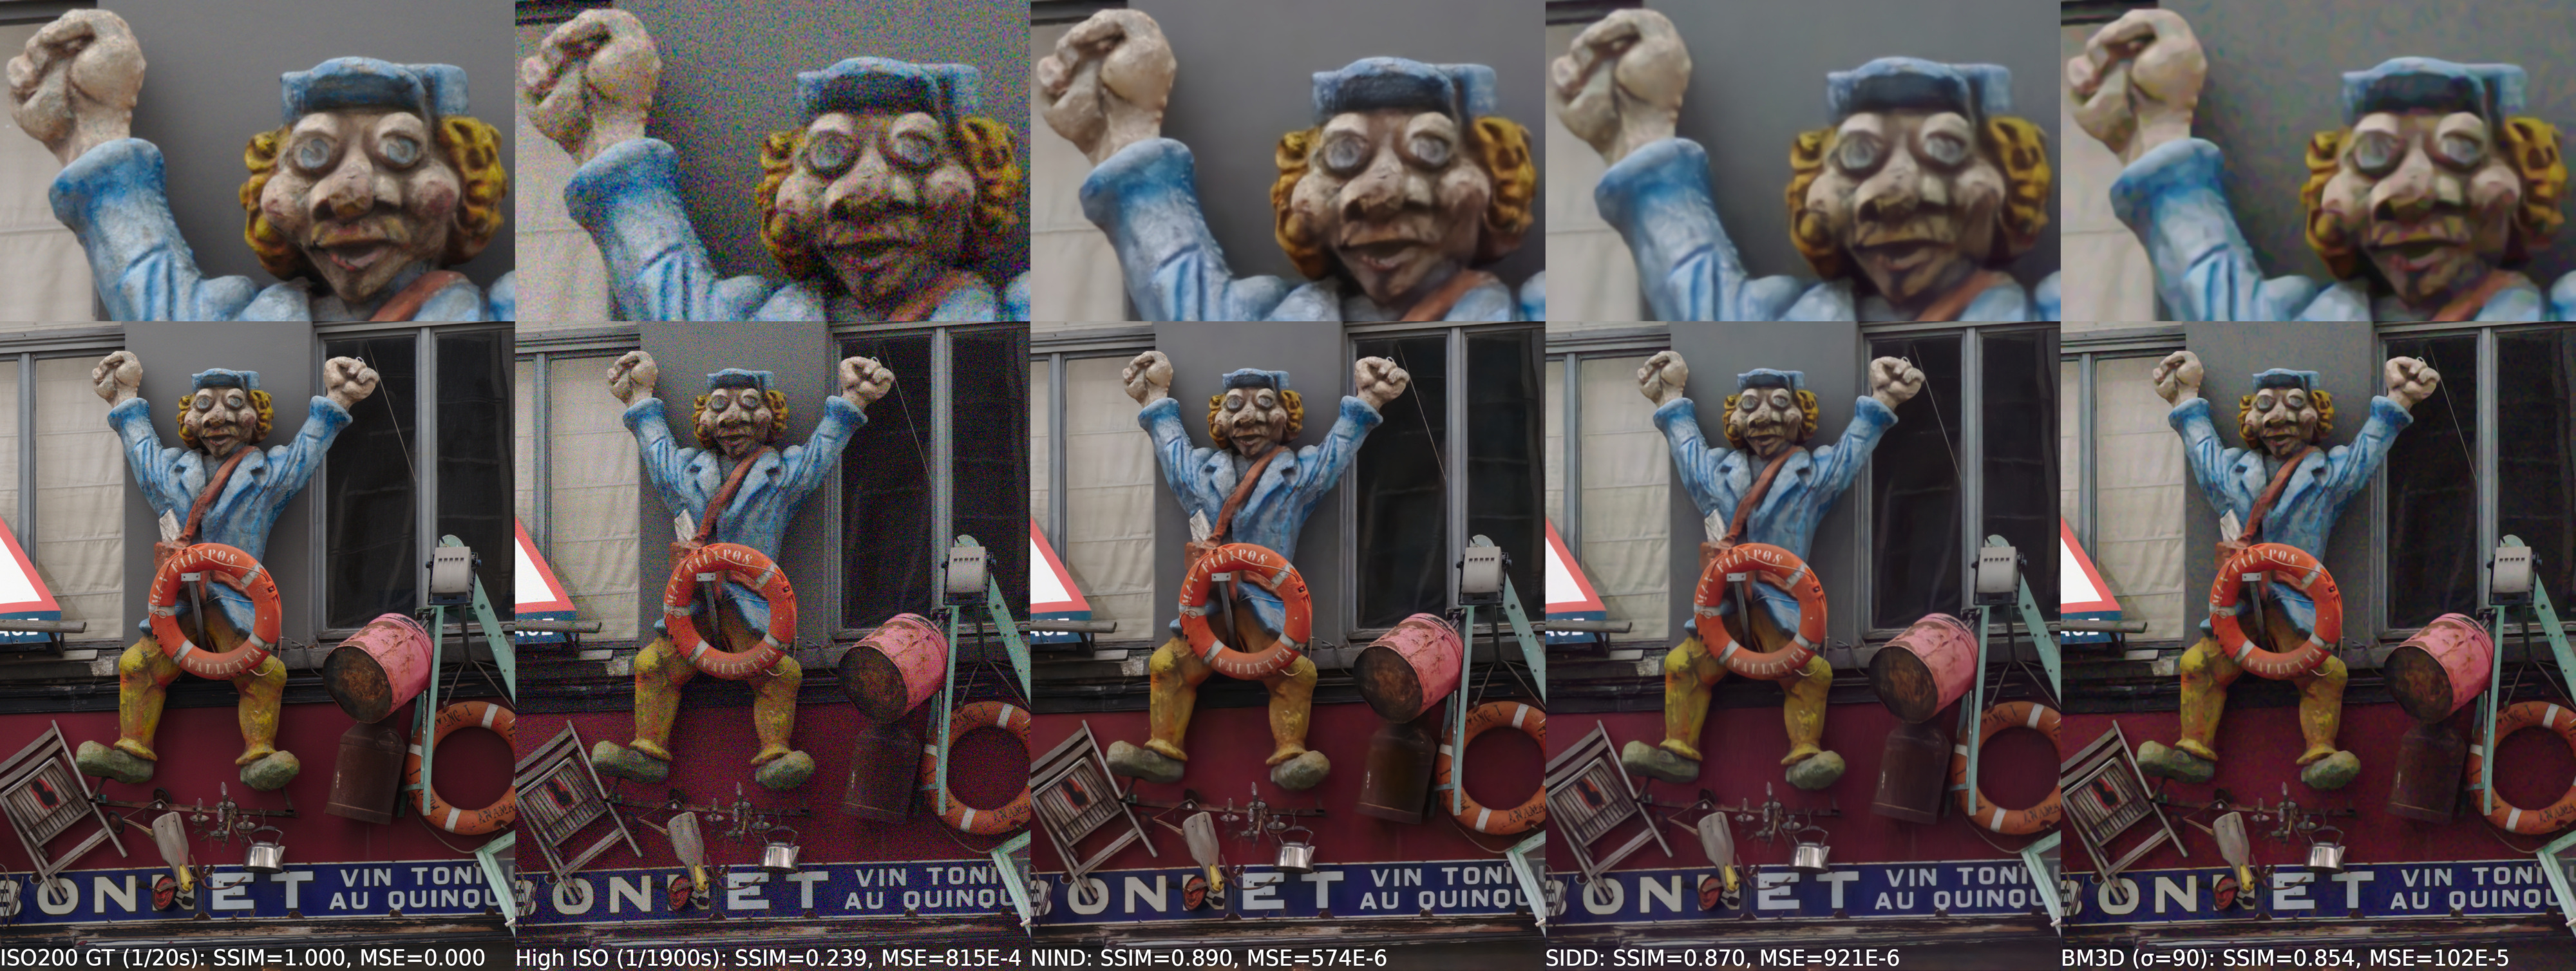
\includegraphics[width=1\linewidth]{gfx/comp/stefantiek.jpg}
\caption[Denoising stefantiek (visual comparison)]{Denoising stefantiek. 1: ISO200 ground-truth (1/20 s), 2: high ISO (1/1900 s), 3: 2 denoised using U-Net model trained with \ac{NIND}, 4: 2 denoised using U-Net model trained with \ac{SIDD} (320-sets), 5: 2 denoised using \ac{BM3D} ($\sigma=90$\footnoteref{sigmanote})}
\label{fig:stefantiek}
\end{figure*}

% \begin{figure}[!htbp]
% \centering
% 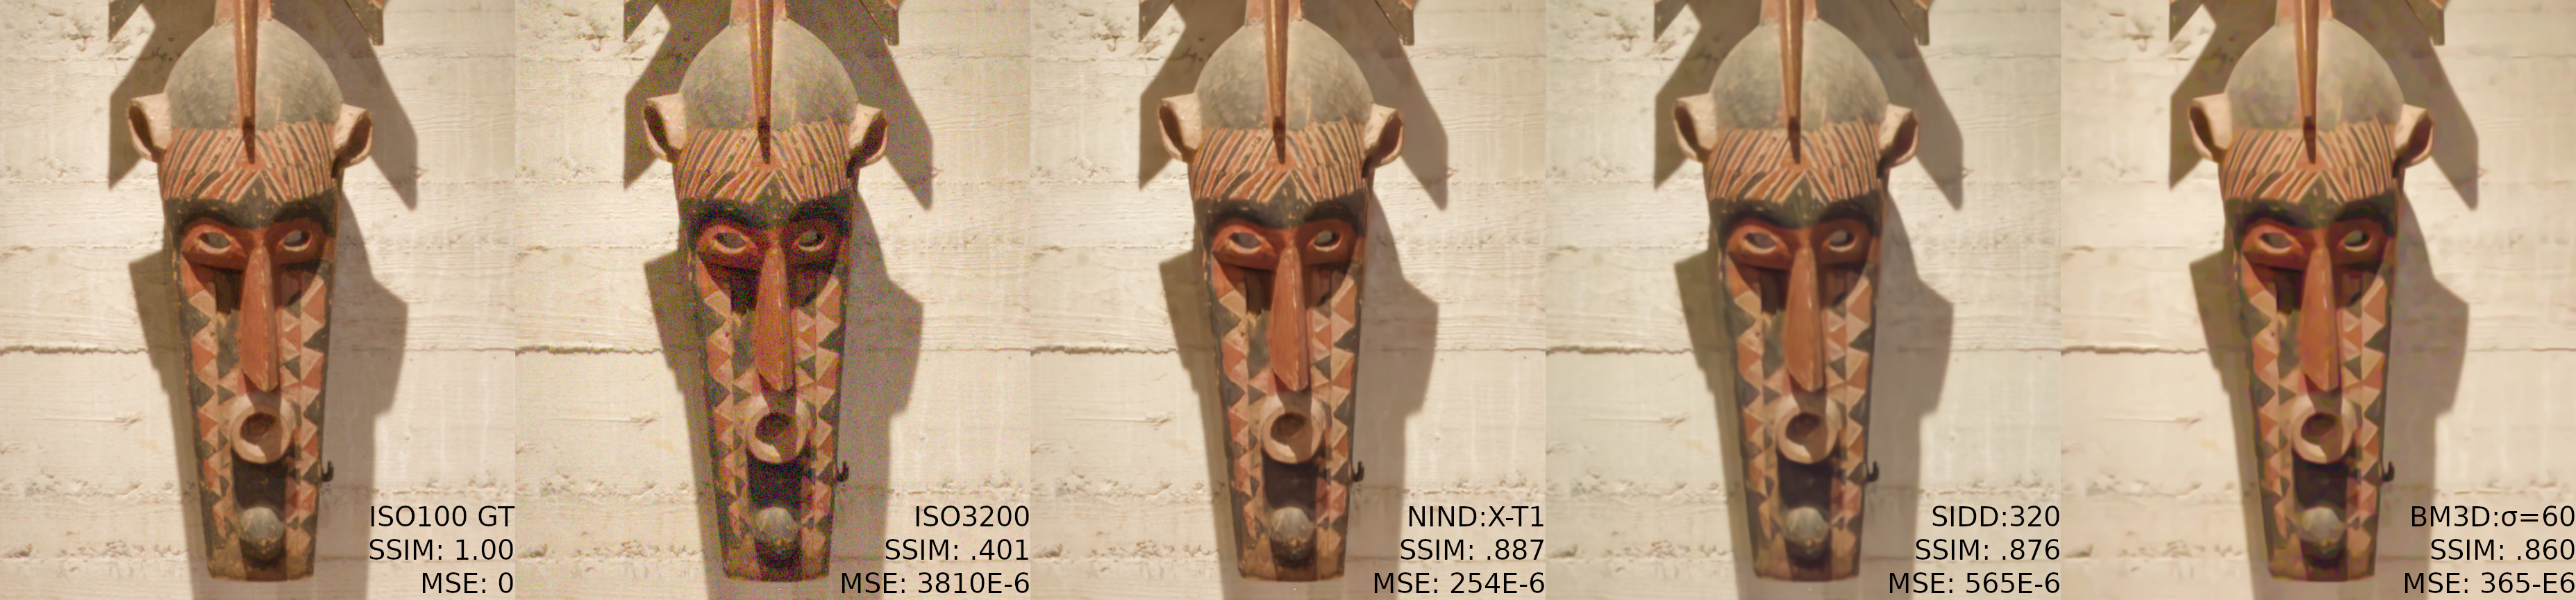
\includegraphics[width=1\linewidth]{../comp/NIND_MuseeL-Bobo-C500D.jpg}
% \caption{Denoising MuseeL-Bobo-C500D. 1: ISO100 ground-truth (4s), 2: ISO3200 (1/10s), 3: 2 denoised using U-Net model trained with \ac{NIND} (X-T1 subset), 4: 2 denoised using U-Net model trained with \ac{SIDD} (320-sets), 5: 2 denoised using BM3D ($\sigma=60$)}
% \label{fig:boboc500dvis}
% \end{figure}

\begin{figure*}[!htbp]
\centering
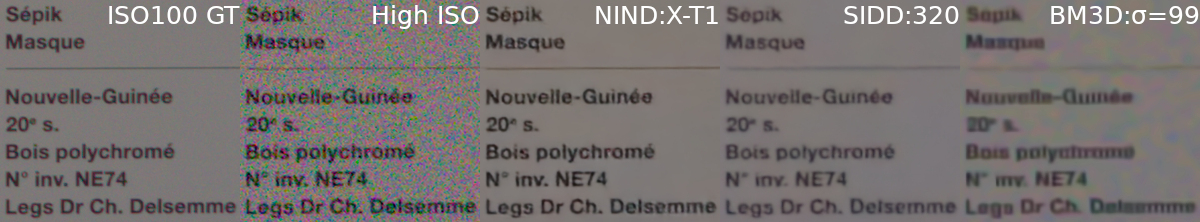
\includegraphics[width=1\linewidth]{gfx/comp/txt.jpg}
\caption[Denoising text present on MuseeL-Sepik-C500D (visual comparison)]{Denoising text present on MuseeL-Sepik-C500D. 1: ISO200 ground-truth (2 s), 2: high ISO (1/30 s), 3: 2 denoised using U-Net model trained with \acs{NIND}:\acs{X-T1}, 4: 2 denoised using U-Net model trained with \ac{SIDD} (320-sets), 5: 2 denoised using \acs{BM3D} ($\sigma=99$\footnoteref{sigmanote})}
\label{fig:text}
\end{figure*}

\begin{figure}[!htbp]
\centering
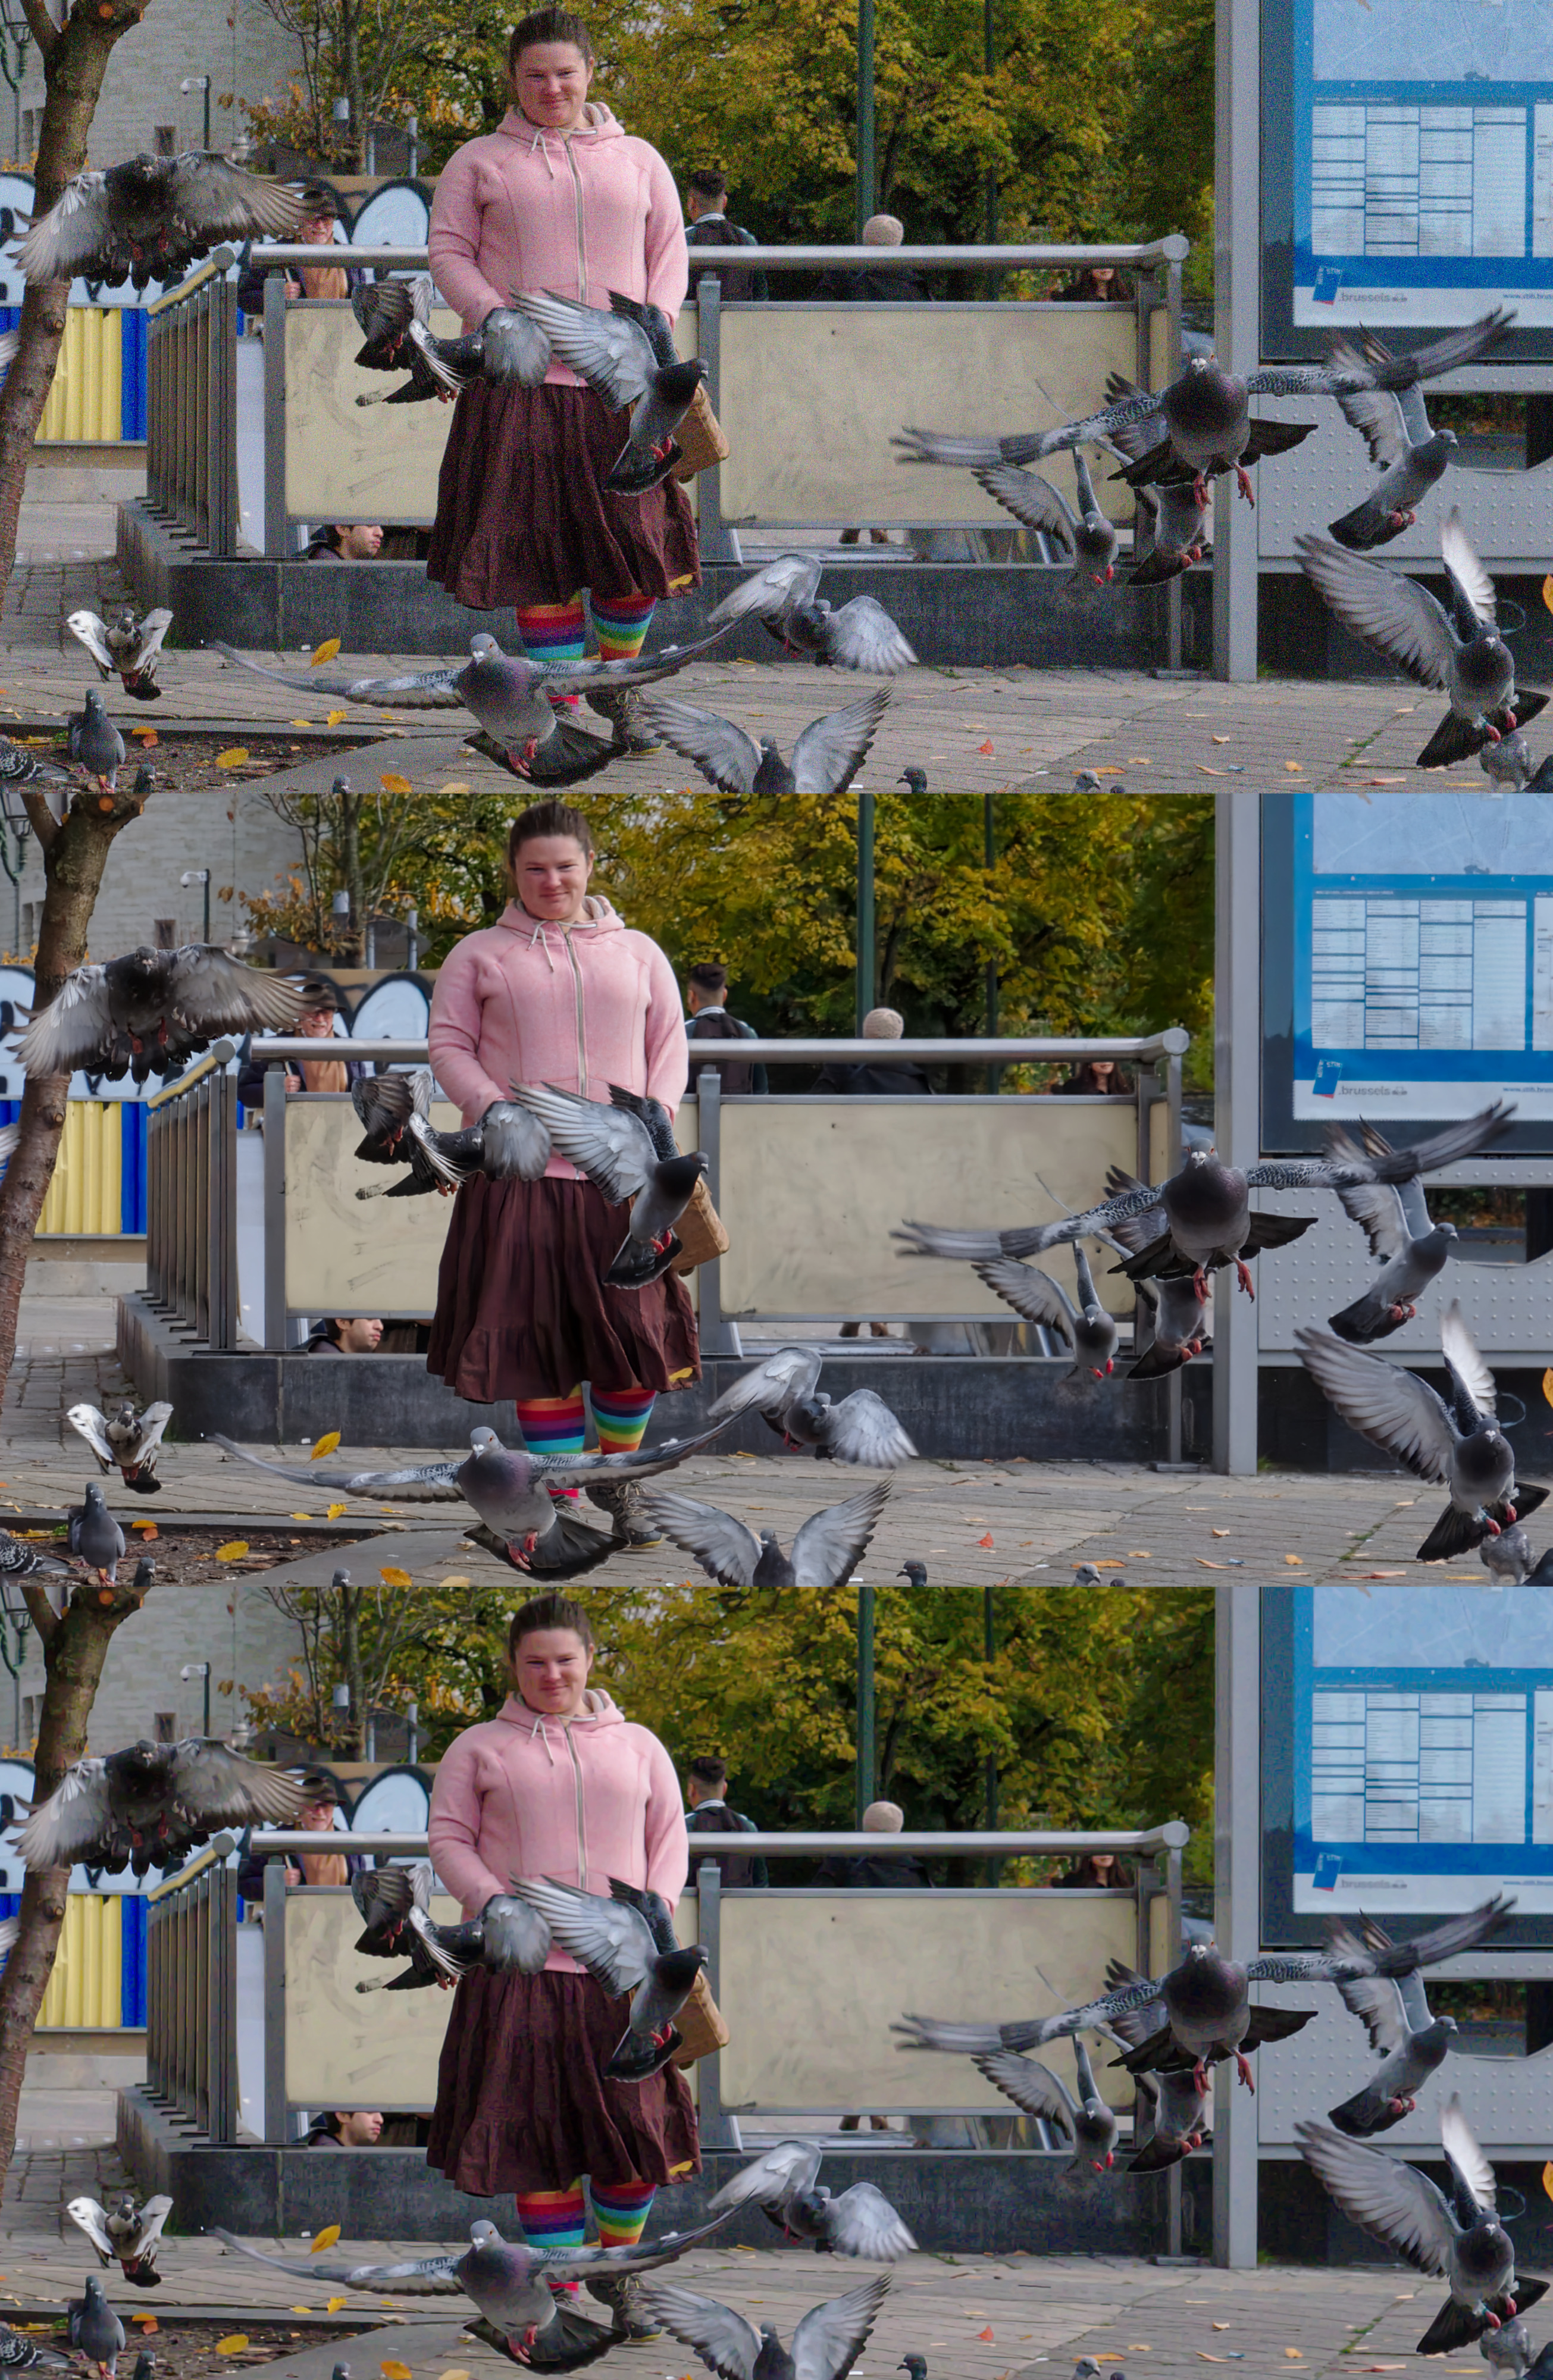
\includegraphics[width=1\linewidth]{gfx/comp/comp-noisy-nind-bm3d30.jpg}
\caption[Denoising of an unpaired "high-speed" image (visual comparison)]{Comparison between a noisy ISO6400 crop (top), one denoised with a model trained on \ac{NIND} (middle), and one on which \ac{BM3D} ($\sigma=30$) has been applied (bottom). Our model appears to perform well on dynamic scenes despite having been trained on static scenes.}
\label{fig:visualpigeons}
\end{figure}


Each network is trained for 48-hours on a GeForce GTX 1080 (11GB). % 77.1% of the time SIDD
Table \ref{tableNINDXT1} shows denoising performance on the Fujifilm X-T1 test pictures. We observe that the model trained on the \ac{NIND} significantly outperforms \ac{BM3D} and that adding training data from the Canon EOS 500D sensor, as well as part of the \ac{SIDD} dataset, does not appear to negatively impact performance. Table \ref{tableNINDXT1onBoboC500D} and Figure \ref{fig:boboc500d} show denoising performance on the scene ``MuseeL-Bobo-C500D", where a model trained only with \ac{NIND}:\ac{X-T1} data performs nearly as well as a model that was also trained with \ac{NIND}:\ac{C500D} data (and so does a model trained with both \ac{NIND} and \ac{SIDD}). Table \ref{tableXT1onC500D} summarizes the average performance of \ac{X-T1}-trained models on ten \ac{C500D} scenes and shows performance which considerably exceeds that of \ac{BM3D} even though the model was generalizing for a different sensor type.

A model trained with only \ac{NIND}:\ac{X-T1} ISO6400 noisy images yields slightly better performance at and around ISO6400, but this comes with a considerable loss of detail at low ISO and the denoising performance becomes poor as the noise level increases. Moreover the model trained on Fujifilm X-T1 ISO6400 images appears not to generalize as well to different sensors as we found it consistently performs worse on the Canon 500D images. These findings suggest that the cost of generalization is acceptably low and therefore a model mostly benefits from learning with different noise levels and sensors.

Reconstructing the noise (Method \ref{exp:nindmakenoise}) as was suggested in \cite{dncnn} typically yields performance below that of BM3D when applied to ISO noise. The difficulty in reconstructing ISO noise was further noticed in an experiment where we mistakenly fed our learning model noisy images as ground-truth 31\% of the time and it still exceeded BM3D performance. This went as far as inverting the clean and noisy crops and still learning an appreciable level of denoising. These findings suggest that a model can easily tolerate some noise in the ground-truth data. Research into this topic \cite{noise2noise}  has been performed to explicitly train models on noisy data and rely on the zero-mean nature of the noise to effectively remove various artificial noise distributions.

Training a model using artificial noise added to ground-truth images (Method \ref{exp:nindart}), as is commonplace in the literature \cite{rednet}\cite{dncnn}, yields the worst performance in our tests.

Figure \ref{fig:text} shows satisfying denoising performance of a model trained on \ac{X-T1} images with text recovered from a \ac{C500D} image. In addition to the aforementioned results based on \ac{SSIM}, we have subjectively tested our \ac{NIND}-trained model on single images which are not part of the dataset. The first such image is that of a dynamic outdoor scene in which a human walks towards a group of pigeons, causing them to disperse in multiple directions. This type of fast, moving scene cannot be included in the dataset due to its dynamic nature and it must be captured with settings that result in a poor quality image; a small aperture (f/11) to focus everywhere, a fast shutter speed (1/1500 s) to capture the flying birds, and a maximum sensor sensitivity (ISO6400) to match the aforementioned settings. Nonetheless, we found the denoised image to be of high quality; we submitted it to the Wikimedia Commons ``Quality Images Candidates" page \cite{qic} and it was subsequently promoted to a ``Quality Image" by Wikimedia Commons reviewers. A crop of the image is provided on Figure \ref{fig:visualpigeons} with a comparison between the noisy version, one denoised with a U-Net model trained on \ac{NIND}, and a version that has been denoised using \ac{BM3D} (with $\sigma=30$ which, on average, yields the highest \ac{SSIM} in our ISO6400 test images). The BM3D version shows significant displeasing artifacts, for example on the skirt and the blue uniform panel on the right, while the model trained on \ac{NIND} smoothed these regions appropriately while retaining a greater level of useful details such as those present on the pigeons' wings.

%%%%%%%%%%%%%%%%%%%%%%%%%%%%%%%%%%%%%%%%%%%%%%%%%%%%%%%%%%%%%%%%%%%%%%%%%%%%%%%%%%%%%%%%%%%%%%%
%%%%%%%%%%%%%%%%%%%%%%%%%%%%%%%%%%%%%%%%%%%%%%%%%%%%%%%%%%%%%%%%%%%%%%%%%%%%%%%%%%%%%%%%%%%%%%%
%%%%%%%%%%%%%%%%%%%%%%%%%%%%%%%%%%%%%%%%%%%%%%%%%%%%%%%%%%%%%%%%%%%%%%%%%%%%%%%%%%%%%%%%%%%%%%%

\section{GAN Denoising}\label{sec:GAN Denoising}

We initially trained denoising networks using the pix2pix approach (the typical use-case is generating photorealistic images from rough sketches) of performing image to image translation using a PatchGAN discriminator and a U-Net generator \cite{pix2pix}. The results were not satisfying even after applying the adjustments mentioned in section \ref{sec:Initial training method}; the PatchGAN would consistently prefer high frequencies and the denoising performance suffered. We thus designed our own HulDisc discriminator and a similar HulbNet generator and tested their individual building blocks in section \ref{sec:Components} before assessing the system as a whole and comparing it to previous approaches in section \ref{sec:System as a whole}.

\subsection{PatchGAN}

We first tried following the pix2pix approach using a PatchGAN discriminator and a U-Net generator \cite{pix2pix} with 1:3 training ratio. The discriminator handles high-frequency details and low-frequencies are handled by the $\ell 1$ loss. We were unable to obtain satisfying performance after experimenting with different loss balances, we found that the denoising performance was subpar to that of \ac{BM3D} and of our previous U-Net network; high-frequencies tend to be exaggerated in low-frequency areas and high frequency details are not properly recovered, often resulting in an overall poor \ac{SSIM} index. Figure \ref{fig:p2p-def} illustrates the denoising performance obtained using a 0.25 $\ell 1$ multiplier.

\begin{figure}[!htbp]
  \begin{center}
    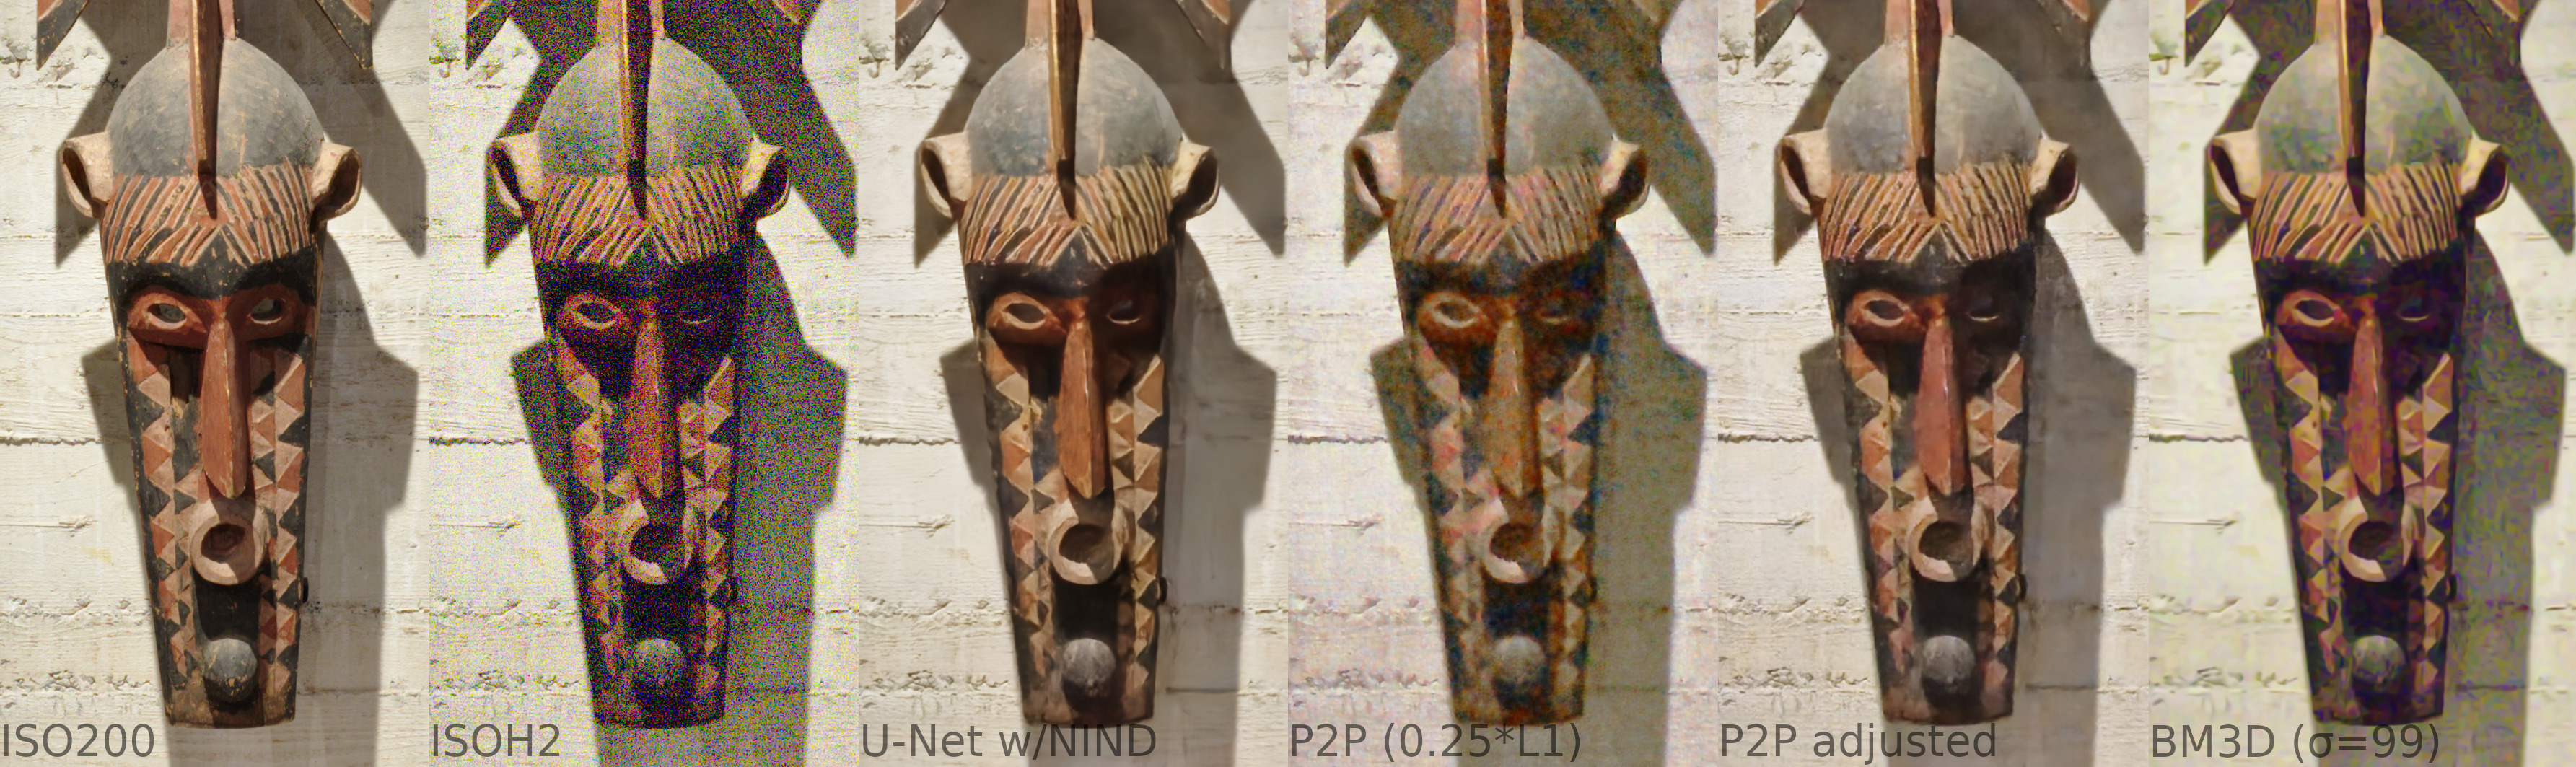
\includegraphics[width=1\linewidth]{gfx/comp/p2p_def.jpg}
    \caption[Initial (c)GAN denoising (visual comparison)]{Comparison of standard pix2pix \cite{pix2pix} applied to image denoising with other methods on a crop from image NIND\_MuseeL-Bobo\_ISOH2. 1: ISO200 ground-truth crop (SSIM: 1.00), 2: ISOH2 noisy crop (SSIM: 0.151), 3: Denoised image with a single U-Net network trained on the \ac{NIND} (SSIM: 0.810), 4: Denoised image with a standard pix2pix network trained on the \ac{NIND} with $0.25\times\ell 1$ (SSIM: 0.672), 5: Denoised image with a pix2pix network trained on the \ac{NIND} with the following adjustments: minimum of 35 iterations with $\text{loss}_\text{SSIM} < 0.125$ before using the discriminator with $\text{loss}_G=0.5 \text{loss}_D + 0.4 \text{loss}_\text{SSIM} + 0.1 \text{loss}_{\ell 1}$ (SSIM: 0.794),6: Denoised with \ac{BM3D} using $\sigma=99$ (SSIM: 0.694)}
    \label{fig:p2p-def}
  \end{center}
\end{figure}

Some improvement were made with careful fine-tuning of the learning environment. We added the \ac{SSIM} loss used in single-network training and tested different balances between the $\ell 1$, \ac{SSIM}, and discriminative losses. We tried training the generator without applying a discriminative loss until a SSIM threshold is met for a given number of consecutive iterations, and we tried training a non conditional network. Figure \ref{fig:p2p-comp-1} shows performance on the "stefantiek" set using different settings on a non conditional network (as well as the baseline network performance without these adjustments). We observe particularly poor performance when the discriminative loss has a high weight (weight\_D = 0.9), as well as when we start using the discriminative loss early on before the generator has learned to properly denoise with the conventional loss functions (min\_SSIM=0.3). The GAN network obtains reasonable performance when the generator is pretrained to achieve a \ac{SSIM} loss of 0.125 to 0.15. The greatest performance shown occurs when the generator has to obtain $\text{loss}_\text{SSIM} < 0.125$ for 35 consecutive iterations before using the discriminator as half of the overall loss. A crop denoised with this model (5) is shown beside one trained with standard pix2pix \ac{cGAN} (4) on Figure \ref{fig:p2p-def}.

\begin{figure}[!htbp]
\centering
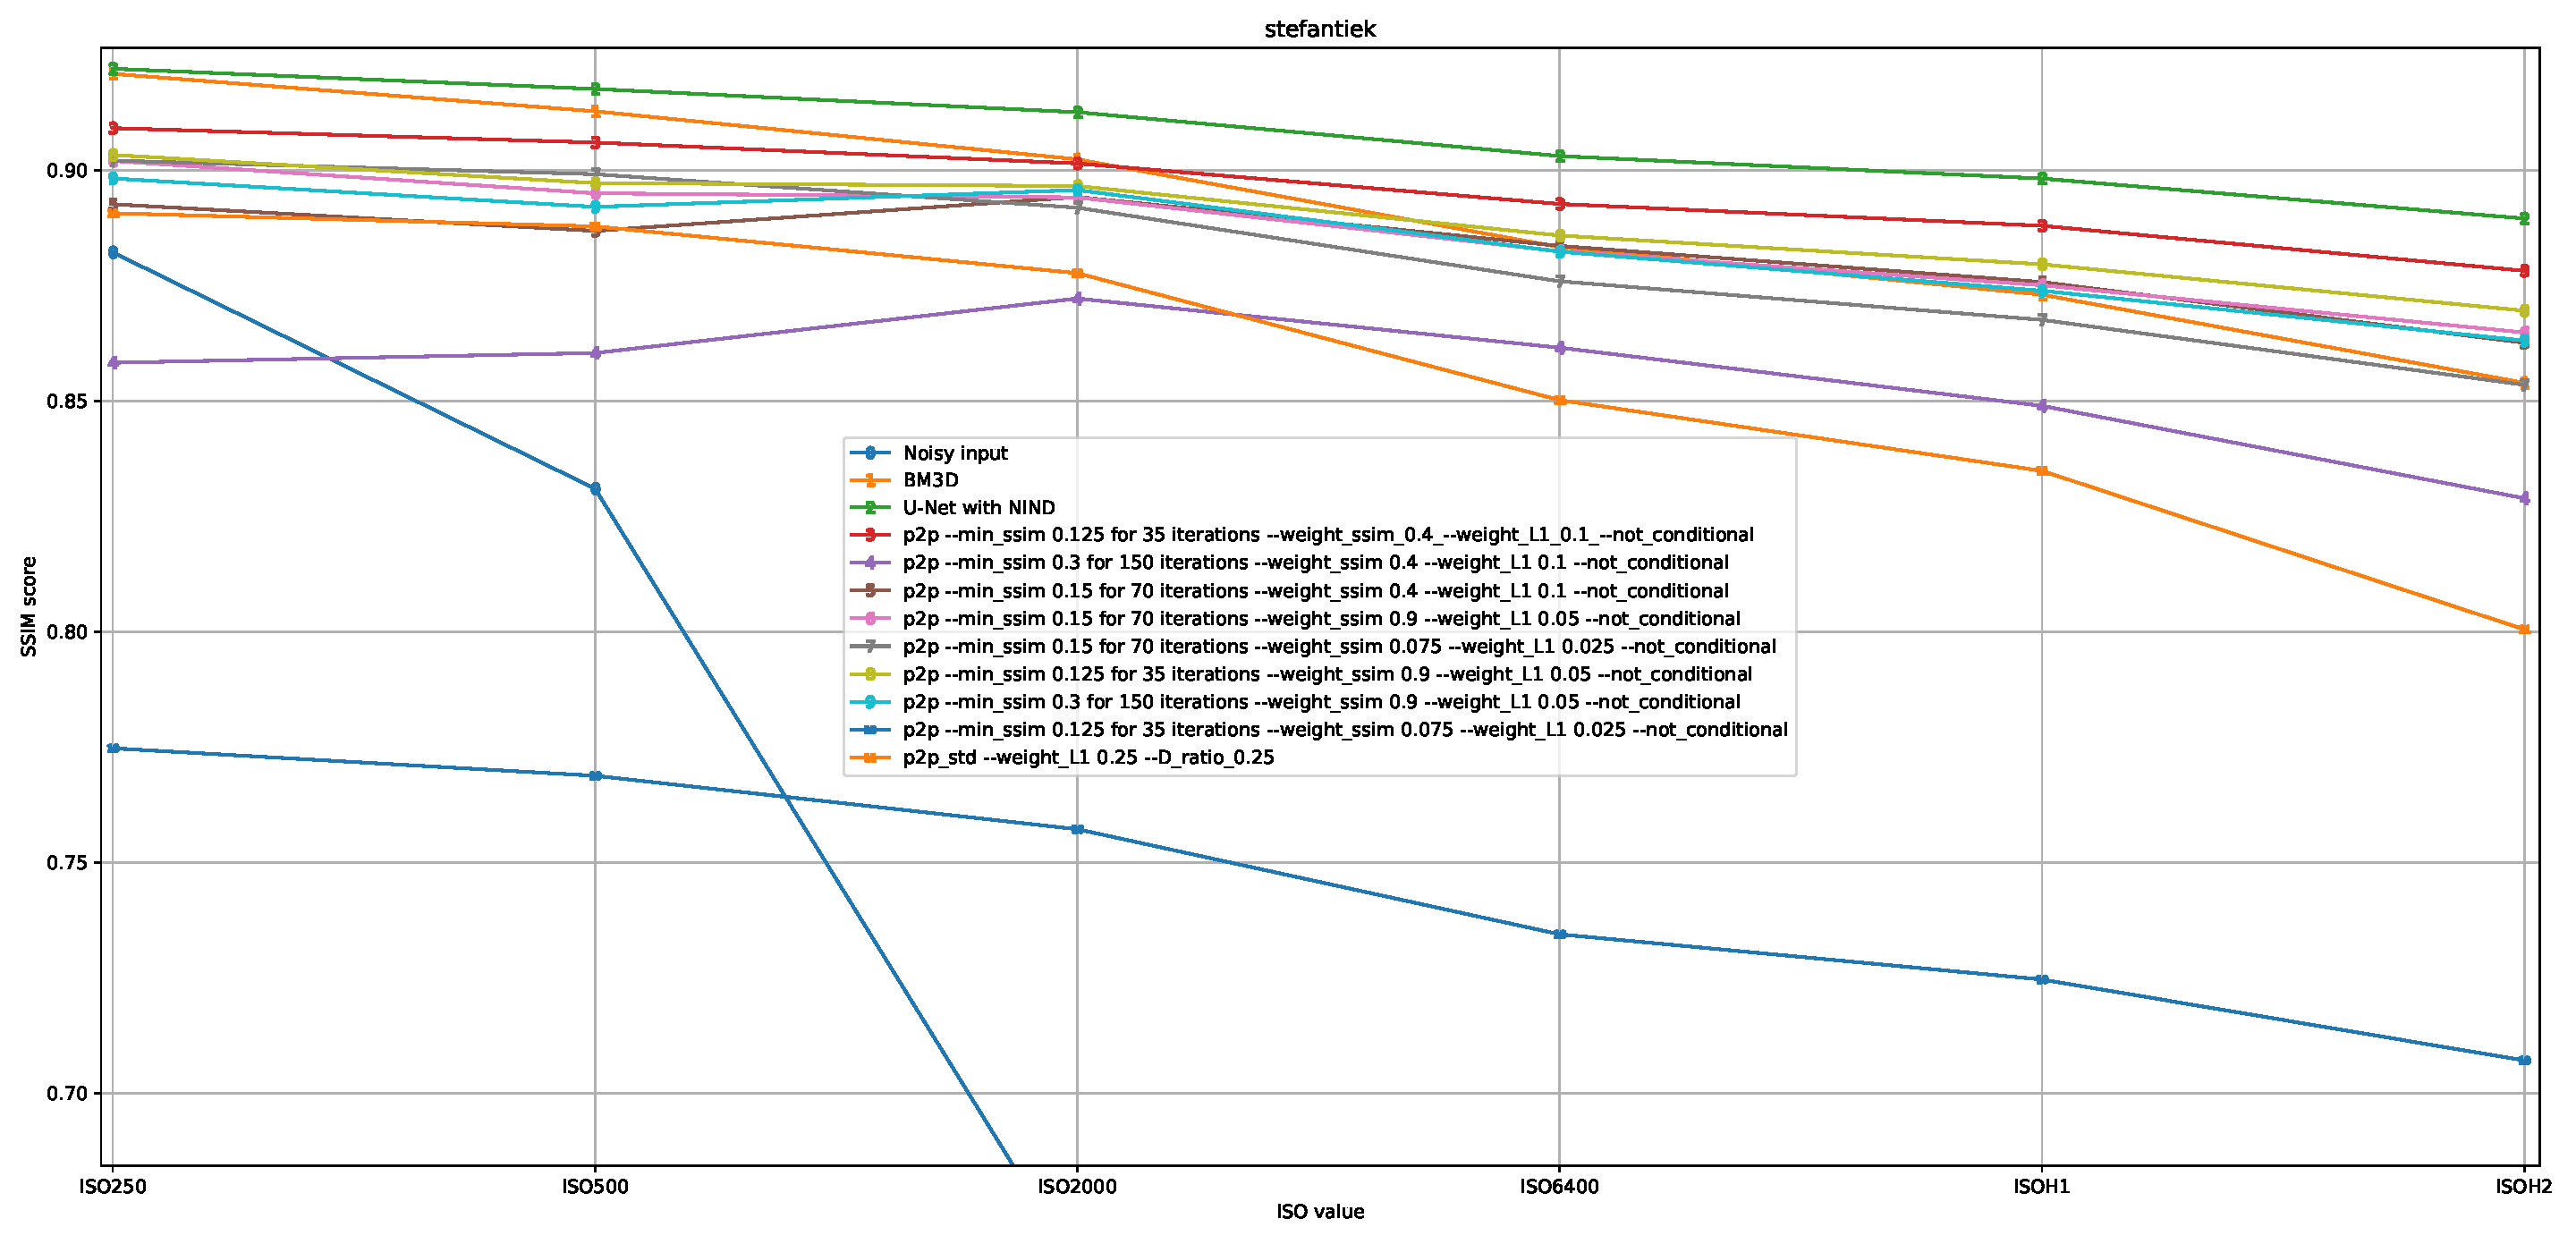
\includegraphics[width=1\linewidth]{gfx/graphs/p2p-comp-1.pdf}
\caption[Denoising performance of \acsp{GAN} on the "stefantiek" set]{Denoising performance of the non conditional GAN with varying weights and schedules on the "stefantiek" set over increased ISO values. The models appear to perform better when they are pre-trained to achieve good performance with the \acs{SSIM} loss before taking the discriminator's feedback into account, and when the discriminator's weight (1 - other weights) does not account for the bulk of the loss function.}
\label{fig:p2p-comp-1}
\end{figure}

\subsection{Our proposed architecture}
\subsubsection{Components}\label{sec:Components}
Our main motivation for designing the "Hul" architectures described in sections \ref{HulbNet} and \ref{HulDisc} is the poor performance obtained with a PatchGAN discriminator; the discriminative network should not focus only on high-frequencies or its feedback becomes corruptive. We also wanted to replace the U-Net generative network which loses too much border that is either easily discriminated against or that does not leave a large enough crop for the discriminator to make up meaningful results. We thus designed both a generator and a discriminator which follow the same design ideas (alas the discriminator is cut in half and thus loses many of the dense connections), and tested specific components for their respective use-cases.
%Network like \cite{pix2pixhd} which processes multiple scales to capture high-frequencies and smooth textures. Instead of dividing up the images into different resolutions or using multiple networks, we followed an approach similar to that of DenseNet \cite{densenet} which concatenates multiple channels together from different layers (as opposed to summing the features \cite{resnet}), allowing layers to contain different types of features captured with different convolutions. Some of the convolutions thus capture a wider receptive field using dilation which has been shown to perform well in image segmentation tasks \cite{multi-scale-dilation}, while other channels focus on local details with standard convolutions.

%At the same time we wanted to replace the U-Net network which loses too much border that is either easily discriminated against or does not leave a large enough crop for the discriminator to make up meaningful results. We thus designed both a generator and a discriminator which follow the same design ideas (alas the discriminator is cut in half and loses many of the dense connections), and tested specific components for their respective use-cases.

The two architectures were trained separately to assess and optimize their individual performance before working together. The generator is typically trained using the same framework as that of section \ref{sec:CNN Denoising}, while the discriminator main tests involve discriminating between clean and noisy crops from the dataset without receiving the conditional input. This test is not as robust as training with the result of a static generator but it allows us to quickly get a preview of the discriminator's performance whereas it would not always be able to learn from scratch given a well trained generator.

\begin{figure}[!htbp]
\centering
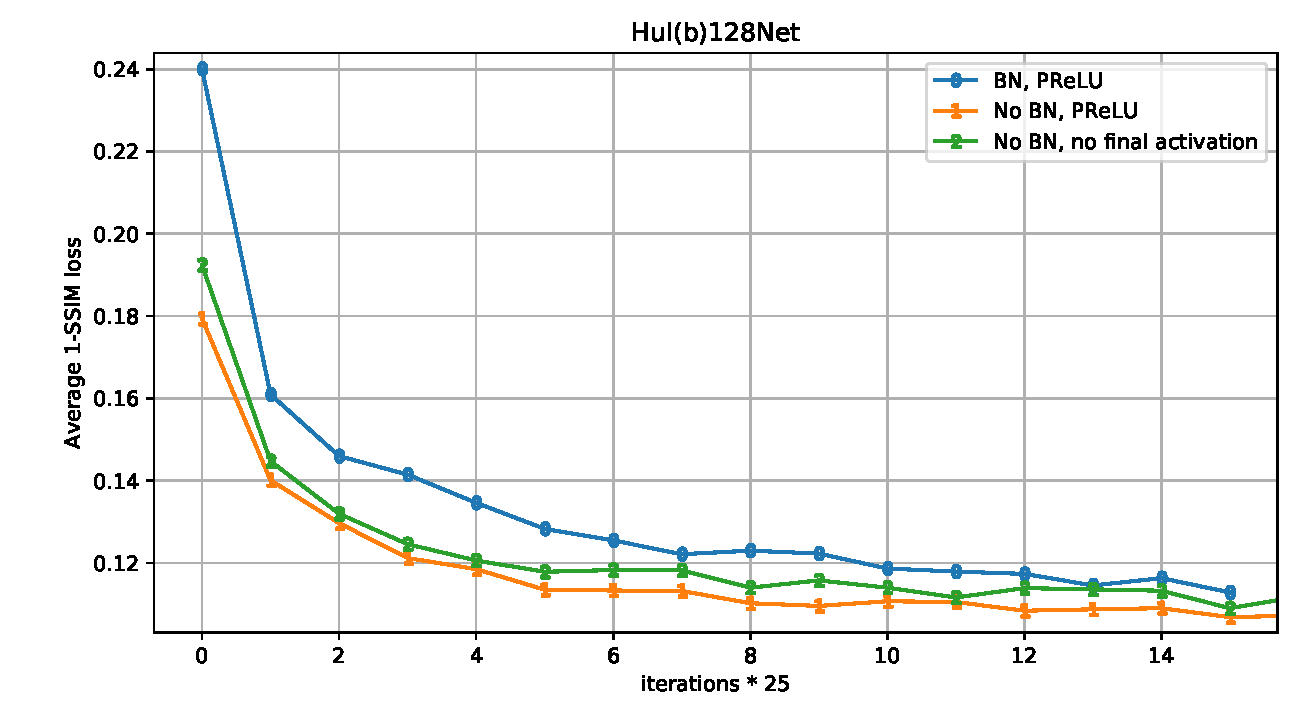
\includegraphics[width=1\linewidth]{gfx/graphs/gen-BN.pdf}
\caption[Generative network learning curve with and without batch normalization]{Generative network learning curve with and without \acl{BN} ("HulbNet"), as well as with neither \ac{BN} nor an activation function. We observe better performance when \acl{BN} is not applied and with the use of a non-linear final activation function.}
\label{fig:gen-BN}
\end{figure}

\acl{BN} appeared to hamper learning on the generative networks, often yielding worse color rendition and lowering the \ac{SSIM} index (which does not appear to be very sensible to color accuracy). We trained a generative network for an epoch with and without batch normalization to finally determine whether \ac{BN} should be removed from the generative network. Figure \ref{fig:gen-BN} shows the resulting learning curve, which allows us to confidently remove \ac{BN} from the generative architecture (we add the letter b such that "HulbNet" denotes a network without \ac{BN}). We also trained a network for an epoch to determine whether not using a final loss function as is sometimes done \cite{dncnn} would yield better performance than \ac{PReLU}, but we found the network performs better with a non-linear activation function.

% TODO fix imbalance
% TODO explicitly mention loss
\begin{figure}[!htbp]
\centering
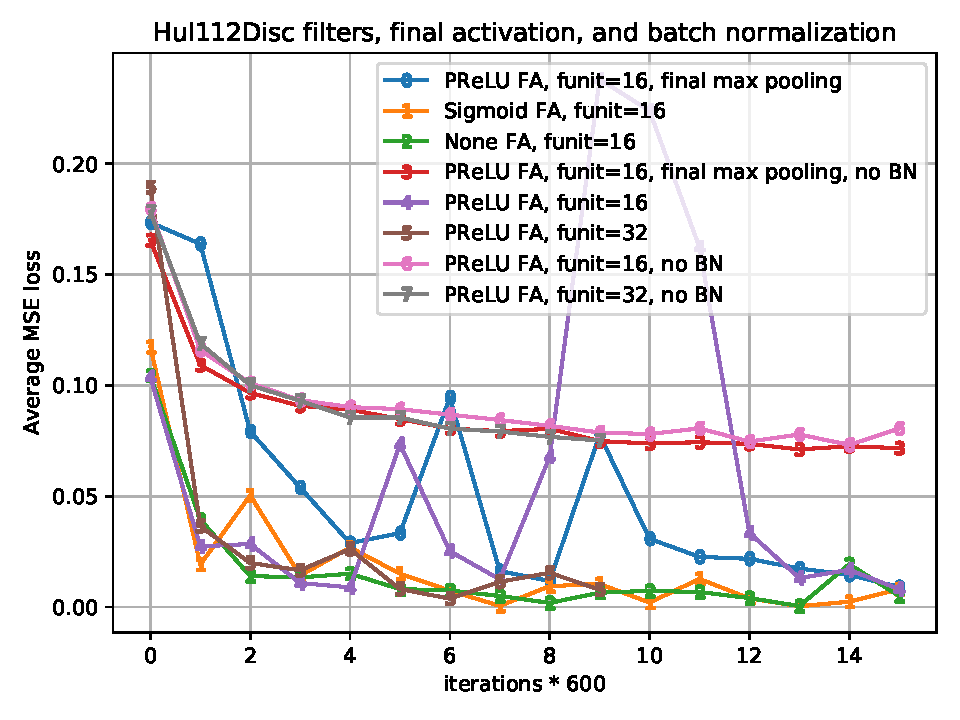
\includegraphics[width=1\linewidth]{gfx/graphs/hul112disc-activ.pdf}
\caption[Discriminative network learning curve with different final activation functions and number of filters]{Discriminative network learning curve with varying final activation functions (FA) and number of filters. We observe that the discriminative network benefits greatly from \ac{BN} and that training stability and performance suffer from not having a sufficient number of filters. One funit denotes the number of filters multiplier (with the first layer outputting two funits). The network is not conditioned and its task is to discriminate whether an image is clean or noisy. The loss is squared therefore a \ac{MSE} of 0.25 is equivalent to guessing 0.5.}
\label{fig:hul112disc-activ}
\end{figure}

% TODO add hulfdisc
Figure \ref{fig:hul112disc-activ} shows the discriminator's learning curve classifying images as either clean or noisy. We observe that \acl{BN} is useful in the case of the discriminator, likely because its job does not entail recreating image fidelity from the input but output a single probability, and \acl{BN} can help when given mini-batches of a single target value (line 3, 6, 7). We observe that the \ac{PReLU} activation function yields sporadically very poor performance on line 0 and 4, but performance is restored with a greater number of filters. Ending the discriminative network with a final max-pooling appears worse than a learned convolution. The different activation functions seem roughly equivalent as they overtake one other over time. Although we observe the importance of using a sufficient number of filters, we cannot conclude an actual number of needed filters from this experiment because the task is simpler than discriminating between real (baseline) and fake (denoised) images, but the real task at hand cannot be accomplished because the discriminator never catches up if there is a large discrepancy between an untrained discriminator and a pre-trained generator.

\begin{figure}[!htbp]
\centering
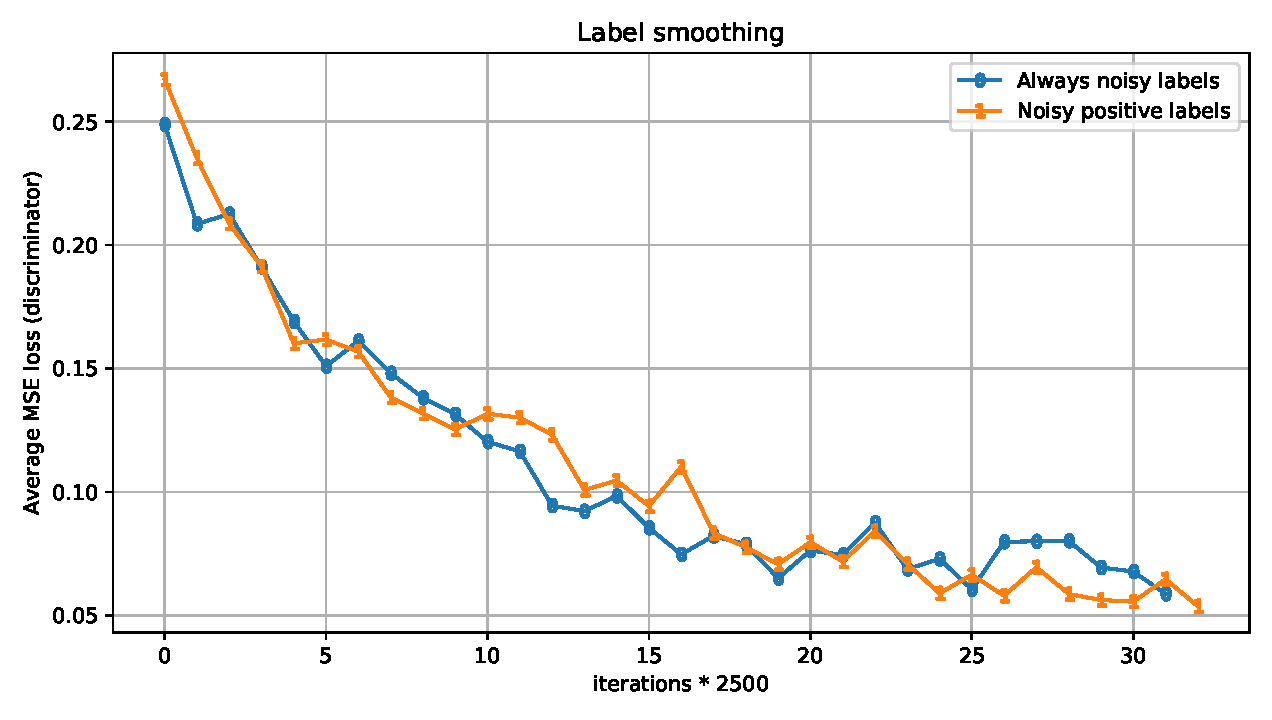
\includegraphics[width=1\linewidth]{gfx/graphs/label-smoothing.pdf}
\caption[Discriminative network performance with noisy labels (always noisy or noisy for positive labels only)]{Discriminative network performance (\ac{MSE} loss) with noisy labels (either always noisy or noisy for positive labels only). The network attempts to discriminate images denoised by a generator which has been trained for three epochs and is continuously being updated (alas without any input from the discriminator). We did not observe a notable difference in performance between the two label smoothing methods.}
\label{fig:label-smoothing}
\end{figure}

Following some incertitude on whether label smoothing should only be applied on positive labels as per \cite{gantechniques} or on all batches used to train the discriminator, we compared the two approaches and show the results on figure \ref{fig:label-smoothing}. The test protocol is different from the previous one in that the discriminator attempts to discriminate against images denoised by a generator which has been pre-trained for three epochs (and is continuously being updated, although it receives no feedback from the discriminator). The results we observed did not seem to differ significantly as the two discriminators would continuously overtake one other.

% switching losses is bad
\subsubsection{System as a whole}\label{sec:System as a whole}

In this section we test different configurations of our "Hul" \ac{cGAN} networks as a whole system. The performance is compared to the previously used configurations as well (U-Net alone and the PatchGAN), and we assess the visual quality of denoised images where it was previously lacking (i.e. noisy face images).

The different types of network present in this experiment are as follow:
\begin{itemize}
  \item Hul is the base name of the network we use
  \item b: no batch normalization
  \item f: more channels as the other dimensions decrease
  \item A number representing the minimum valid input size
  \item Disc for discriminators or Net for generators
\end{itemize}

\begin{figure}[!htbp]
\centering
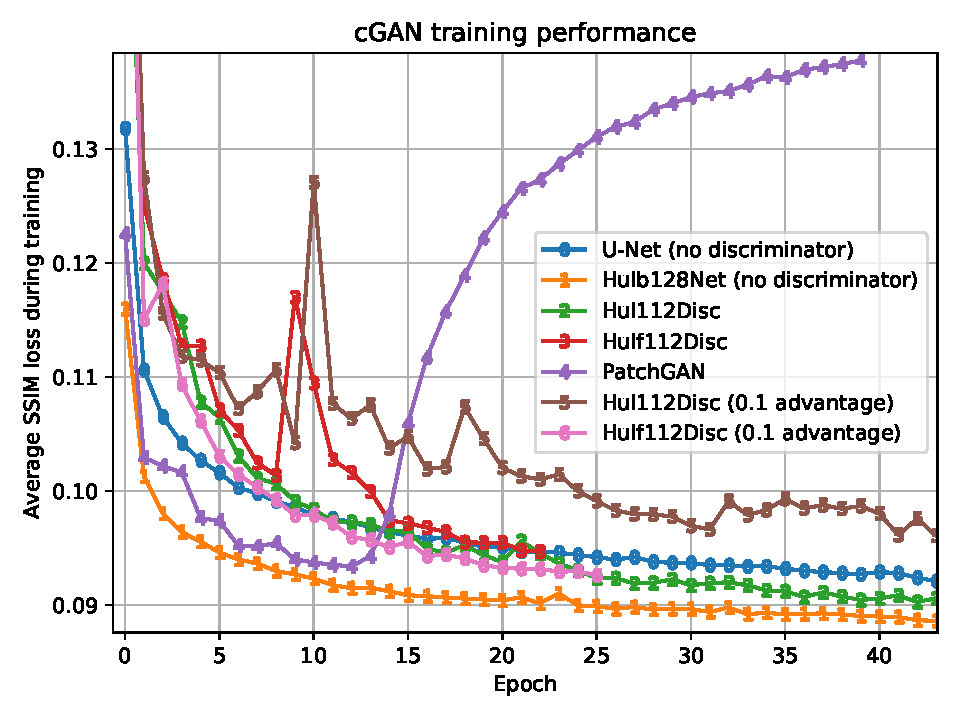
\includegraphics[width=1\linewidth]{gfx/graphs/cgan-comp.pdf}
\caption[cGAN training performance comparison]{
cGAN training performance comparison. 0: The U-Net from section experiment \ref{exp:nindxt1}, 1: Hulb128Net (without a discriminator). The following networks all use the Hulb128Net generator and a specified discriminator. 2: Hul112Disc, 3: Hulf112Disc (more filters as the network shrinks), 4: PatchGAN \cite{pix2pix}, 5: Hul112Disc which learns 10\% more often than the generator, 6: Hulf112Disc which learns 10\% more often than the generator. We observe that the increased number of filters (Hulf112Disc) destabilizes the discriminator, but performance is restored when the discriminator has more time to learn. On the other hand, giving more time to a discriminator that does not have as much capacity provides worse feedback and the result of the generator suffers. The PatchGAN's performance degenerates quickly, and the Hulb128Net alone offers greater performance than that of U-Net but further analysis shows that the \acs{cGAN} denoised images are visually superior. The \acs{SSIM} training loss is shown. Although \acs{SSIM} is not a meaningful enough factor on its own because the network could recreate a structurally different yet visually pleasing image, it provides an approximate indicator of performance and learning.}
\label{fig:cgan-comp}
\end{figure}

\begin{figure}[!htbp]
\centering
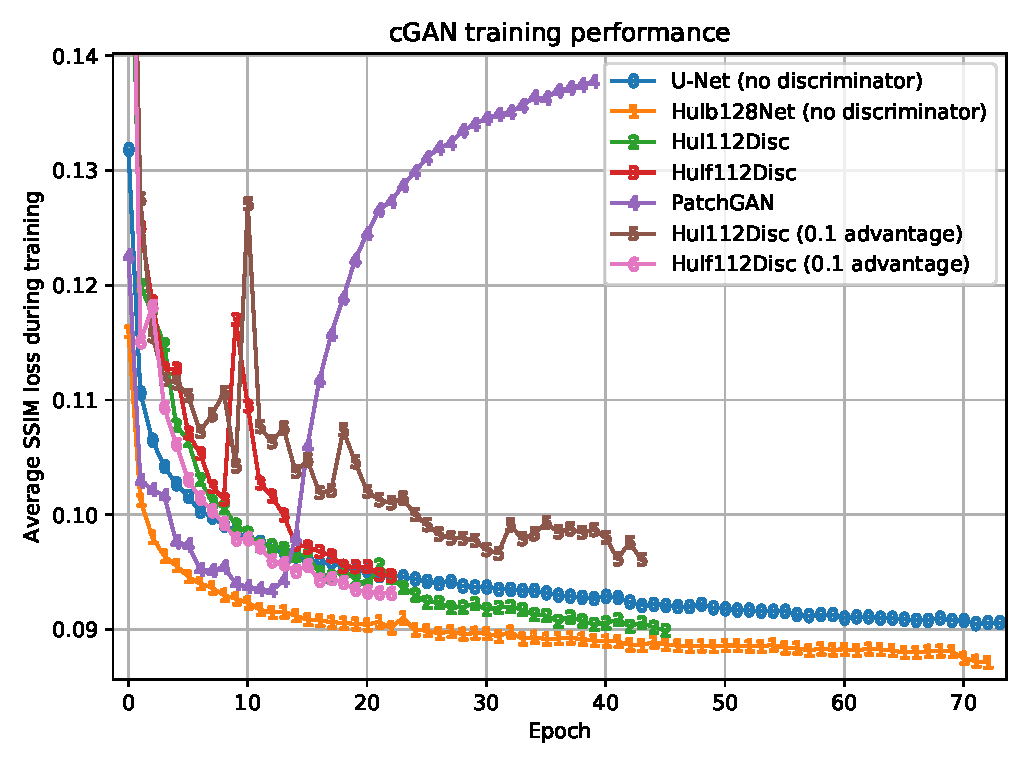
\includegraphics[width=1\linewidth]{gfx/graphs/cgan-comp-longer.pdf}
\caption[cGAN training performance comparison (zoomed-out)]{
cGAN training performance comparison. This is the same graph as Figure \ref{fig:cgan-comp} zoomed out to show that the networks that were trained for longer benefit greatly from the additional time and exceed the performance of a single U-Net generator which maxes out at \acs{SSIM} index=0.902}
\label{fig:cgan-complonger}
\end{figure}

% generate faces, graph on an image
% on:


The networks' training performance is shown on figures \ref{cgan-comp} and \ref{cgan-complonger}. The baseline is a single generative U-Net network, and we also trained a single Hulb128Net network. The Hulb128Net network appears to perform better than the U-Net of our previous experiments. 

Using our HulbNet generative network and HulDisc discriminative network and the training method described in section \ref{sec:Adopted training method}  

TODO (in-progress): HulbNet w/ HulDisc, HulbNet w/PatchGAN, HulbNet w/HulfDisc, HulbNet alone, HulbNet w/ HulDisc with 0.1 advantage

(mention that training with weight\_D >= 0.95 is not stable enough) 

TODO: discriminator\_advantage

TODO conditional vs not conditional

TODO invert probabilities

TODO higher - lower weights

TODO 
